\documentclass[11pt]{article}
\usepackage[utf8]{inputenc}
\usepackage[T1]{fontenc}
\usepackage{lmodern}
\usepackage{amsmath,amssymb,amsthm}
\usepackage{booktabs}
\usepackage{graphicx}
\usepackage[margin=1in]{geometry}
\usepackage{authblk}
\usepackage{natbib}
\usepackage[hidelinks]{hyperref}
\usepackage{microtype}
\usepackage{xcolor}
\emergencystretch=2em
\newcommand{\TODO}[1]{\textcolor{red}{[TODO: #1]}}
\newcommand{\NUM}[1]{#1} % filled from results

% Preprint toggle: build with  pdflatex "\def\PREPRINTMODE{1}\documentclass[11pt]{article}
\usepackage[utf8]{inputenc}
\usepackage[T1]{fontenc}
\usepackage{lmodern}
\usepackage{amsmath,amssymb,amsthm}
\usepackage{booktabs}
\usepackage{graphicx}
\usepackage[margin=1in]{geometry}
\usepackage{authblk}
\usepackage{natbib}
\usepackage[hidelinks]{hyperref}
\usepackage{microtype}
\usepackage{xcolor}
\emergencystretch=2em
\newcommand{\TODO}[1]{\textcolor{red}{[TODO: #1]}}
\newcommand{\NUM}[1]{#1} % filled from results

% Preprint toggle: build with  pdflatex "\def\PREPRINTMODE{1}\documentclass[11pt]{article}
\usepackage[utf8]{inputenc}
\usepackage[T1]{fontenc}
\usepackage{lmodern}
\usepackage{amsmath,amssymb,amsthm}
\usepackage{booktabs}
\usepackage{graphicx}
\usepackage[margin=1in]{geometry}
\usepackage{authblk}
\usepackage{natbib}
\usepackage[hidelinks]{hyperref}
\usepackage{microtype}
\usepackage{xcolor}
\emergencystretch=2em
\newcommand{\TODO}[1]{\textcolor{red}{[TODO: #1]}}
\newcommand{\NUM}[1]{#1} % filled from results

% Preprint toggle: build with  pdflatex "\def\PREPRINTMODE{1}\documentclass[11pt]{article}
\usepackage[utf8]{inputenc}
\usepackage[T1]{fontenc}
\usepackage{lmodern}
\usepackage{amsmath,amssymb,amsthm}
\usepackage{booktabs}
\usepackage{graphicx}
\usepackage[margin=1in]{geometry}
\usepackage{authblk}
\usepackage{natbib}
\usepackage[hidelinks]{hyperref}
\usepackage{microtype}
\usepackage{xcolor}
\emergencystretch=2em
\newcommand{\TODO}[1]{\textcolor{red}{[TODO: #1]}}
\newcommand{\NUM}[1]{#1} % filled from results

% Preprint toggle: build with  pdflatex "\def\PREPRINTMODE{1}\input{main}"  for a
% line-numbered bioRxiv preprint; default (0) is the clean submission build.
\providecommand{\PREPRINTMODE}{0}
\ifnum\PREPRINTMODE=1 \usepackage[switch]{lineno}\fi

\theoremstyle{plain}
\newtheorem{proposition}{Proposition}
\theoremstyle{remark}
\newtheorem{remark}{Remark}

\title{\bfseries Metric-consistent neural networks for genomic prediction and
selection: a standardized-MSE Pearson loss, affine calibration, and
selection-aware evaluation}

\author[1,2]{Gr\'egory Beurier\thanks{Corresponding author: \texttt{gregory.beurier@cirad.fr}}}
\author[1,2]{Denis Cornet}
\author[1,2]{Lauriane Rouan}
\author[1,2]{David Cros}
\affil[1]{CIRAD, UMR AGAP Institut, Montpellier, France}
\affil[2]{UMR AGAP Institut, Univ Montpellier, CIRAD, INRAE, Institut Agro, Montpellier, France}
\date{\ifnum\PREPRINTMODE=1 \textit{Preprint --- not peer-reviewed} \quad\textbullet\quad \today\else\today\fi}

\begin{document}
\maketitle
\ifnum\PREPRINTMODE=1 \linenumbers \fi

\begin{abstract}
\noindent
\input{abstract_body.tex}
\end{abstract}

\section{Introduction}

Genomic selection \citep{meuwissen2001} predicts the genetic merit of candidate
individuals from genome-wide markers, and has become central to modern plant and
animal breeding \citep{heffner2009,jannink2010,desta2014}. The dominant
parametric baseline, genomic best linear unbiased prediction
(GBLUP)/ridge-regression BLUP \citep{vanraden2008,endelman2011}, is increasingly
complemented by machine-learning and deep-learning predictors
\citep{ma2018deepgs,wang2023dnngp,montesinos2021review,montesinos2021power}.
Whether deep learning improves on GBLUP remains dataset-dependent: recent
comparisons find that neither systematically dominates, and that outcomes hinge
on tuning, architecture and the choice of evaluation metric
\citep{montesinos2025dlgblup}.

That last point is the subject of this paper. Genomic predictors are trained, by
near-universal default, to minimize the mean squared error (MSE). But they are
\emph{assessed} with the Pearson correlation $r$ between predicted and observed
phenotypes --- the ``predictive ability'' reported in essentially every genomic
prediction study \citep{crossa2010} --- and they are \emph{used} to rank
candidates and select the best ones. There is therefore a systematic mismatch
between the training objective and one of the principal metrics used to evaluate
genomic prediction. More importantly, neither MSE nor Pearson correlation is
identical to the ranking problem ultimately faced in selection.
\citet{waldmann2019} showed that selecting a model by $r$ can disagree with
selecting it by MSE or $R^2$. \citet{ornella2014} argued that $r$ is a poor guide
to performance in the tails of the distribution, where selection actually
operates, and evaluated the recovery of the best $\alpha\in\{10,\dots,40\}\%$ of
individuals. \citet{blondel2015} reframed genomic selection as a ranking problem,
introduced NDCG from information retrieval as an accuracy measure, and reported
that $r$ correlates poorly with ranking quality.

If correlation is the target, why not train for it directly? A recent
convolutional architecture for genomic selection states plainly that ``Pearson
correlation cannot be set as the loss function'' and substitutes a family of
$L_p$ losses \citep{pnngs2024}. We show this premise is false. The Pearson
correlation \emph{is} a loss --- a standardized MSE --- and training with it is
both well posed and numerically stable. The remaining objection to a correlation
loss, that it ignores scale and offset, is real but easily and provably remedied
by an affine recalibration applied after training.

The empirical question therefore has a simple three-stage structure: compare
the usual MSE-trained raw predictions with Pearson-trained raw predictions to
measure correlation alignment, then calibrate the Pearson outputs on validation
data to recover phenotypic scale, and finally evaluate separately whether
correlation-aligned training changes upper-tail selection. Figure~\ref{fig:loss}
carries this structure through to the headline result.

\paragraph{Contributions.}
\begin{enumerate}
\item \textbf{A standardized-MSE Pearson loss (Section~\ref{sec:prop1}).} We give
the exact identity $\mathrm{MSE}(z_y,z_{\hat y}) = 2(1-r)$ and use it as a stable,
differentiable training objective, verified numerically (to single-precision
tolerance for the loss; to float64 machine precision for the calibration identity).
\item \textbf{Affine calibration with a closed form
(Section~\ref{sec:prop2}).} We prove that the optimal post-hoc affine map yields
residual error $\sigma_y^2(1-r^2)$ on the fitting sample and restores scale and
offset while preserving $r$ and rankings whenever the fitted slope is positive.
\item \textbf{Mini-batch analysis (Section~\ref{sec:prop3}).} We show the
mini-batch Pearson loss is a biased surrogate for the global objective and
quantify the effect of batch size empirically.
\item \textbf{A reproducible, selection-aware benchmark
(Sections~\ref{sec:methods}--\ref{sec:results}).} Across \NUM{101}
trait--datasets from \NUM{12} panels/sources spanning 10 species, with architecture, splits and tuning held
fixed so that only the loss changes, we report both predictive and
selection-oriented metrics, a confirmatory mixed-model analysis, and a
meta-analysis of \emph{when} correlation-consistent training helps. All data are
public and all code, splits and tuned configurations are released.
\end{enumerate}

\noindent We do not claim that a Pearson loss is uniformly superior to MSE; that
would be false. We provide a principled, reproducible framework for training,
calibrating and evaluating neural genomic predictors by treating predictive correlation,
phenotypic scale and selection as related but distinct objectives.

\section{Theory}\label{sec:theory}
Throughout, $y,\hat y\in\mathbb{R}^n$, with sample means $\bar y,\bar{\hat y}$ and
population variances $\sigma_x^2 = \tfrac1n\sum_i (x_i-\bar x)^2$. The Pearson
correlation is $r=r(y,\hat y)=\tfrac1n\sum_i z_{y,i} z_{\hat y,i}$ where
$z_{x,i}=(x_i-\bar x)/\sigma_x$ is the standardized variable.

\subsection{The Pearson loss is a standardized MSE}\label{sec:prop1}
\begin{proposition}\label{prop:1}
For non-degenerate $y,\hat y$ (i.e.\ $\sigma_y,\sigma_{\hat y}>0$),
\[
\mathrm{MSE}(z_y,z_{\hat y}) \;=\; \tfrac1n\sum_{i=1}^n (z_{y,i}-z_{\hat y,i})^2
\;=\; 2\,(1-r).
\]
Consequently $1-r = \tfrac12\,\mathrm{MSE}(z_y,z_{\hat y})$, and minimizing the
standardized MSE is exactly maximizing the Pearson correlation.
\end{proposition}
\begin{proof}
Expanding the square,
$\tfrac1n\sum_i (z_{y,i}-z_{\hat y,i})^2
= \tfrac1n\sum_i z_{y,i}^2 - 2\tfrac1n\sum_i z_{y,i} z_{\hat y,i}
+ \tfrac1n\sum_i z_{\hat y,i}^2 = 1 - 2r + 1 = 2(1-r)$,
because $\tfrac1n\sum_i z_{x,i}^2 = 1$ by construction and
$\tfrac1n\sum_i z_{y,i} z_{\hat y,i}=r$.
\end{proof}
This gives the loss $\mathcal{L}_{\mathrm{P}}(\hat y,y) = 1-r(\hat y,y)$,
implemented directly with a small $\varepsilon$ guarding the standard-deviation
denominators and numerically equivalent to
$\tfrac12\,\mathrm{MSE}(z_y,z_{\hat y})$. It is differentiable everywhere
$\sigma_{\hat y}>0$; we verify the gradient against finite differences and verify
the identity to single-precision tolerance in Section~\ref{sec:res-numerical}. The
negative-correlation loss $-r$ differs from $\mathcal{L}_{\mathrm{P}}$ by a
constant and has identical gradients.

\begin{figure}[tbp]\centering
\IfFileExists{figures/fig1_geometry.pdf}{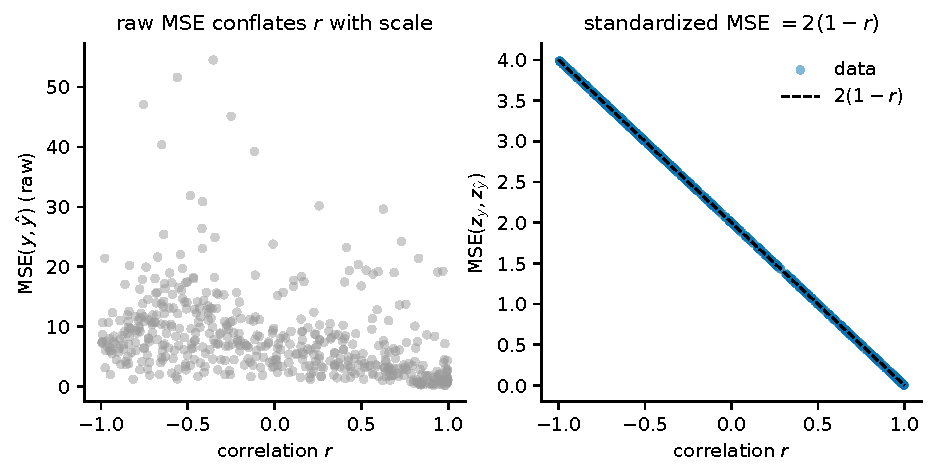
\includegraphics[width=\linewidth]{figures/fig1_geometry.pdf}}{}
\caption{Geometry of the standardized-MSE / Pearson identity (Proposition~\ref{prop:1}).}
\label{fig:geometry}
\end{figure}

\subsection{Affine calibration restores scale without changing rank}\label{sec:prop2}
Correlation is invariant to strictly increasing affine transformations of $\hat
y$: a model trained on $\mathcal{L}_{\mathrm{P}}$ controls the \emph{shape} of the
prediction but not its scale or offset. This is corrected exactly and cheaply.
\begin{proposition}\label{prop:2}
Let $p\in\mathbb{R}^n$ be raw predictions and $r=r(y,p)$. The affine map
$\tilde y = a\,p+b$ minimizing $\tfrac1n\sum_i (a p_i + b - y_i)^2$ has
\[
a^\star = \frac{\mathrm{cov}(y,p)}{\mathrm{var}(p)},\qquad
b^\star = \bar y - a^\star\,\bar p,\qquad
\mathrm{MSE}_{\min} = \sigma_y^2\,(1-r^2).
\]
If $a^\star>0$, the map is strictly increasing and hence preserves $r$, the
Spearman correlation, and every top-$k$/ranking quantity, while setting the
calibration slope to $1$ and intercept to $0$.
\end{proposition}
\begin{proof}
Ordinary least squares for a single predictor gives $a^\star,b^\star$ as stated;
the minimized residual variance of simple linear regression is
$\sigma_y^2(1-r^2)$. A strictly increasing transform preserves the order of $p$
and leaves correlation-type and rank-based statistics unchanged.
\end{proof}
We fit $(a^\star,b^\star)$ on held-out validation predictions (never on the test
set) and apply them to the test predictions. Isotonic regression provides a
monotone non-linear alternative when the raw-vs-true relationship is monotone but
curved. A positive affine map preserves $r$; a negative affine slope changes its
sign, and nonlinear isotonic calibration can change its magnitude. Calibration
can nonetheless improve RMSE, bias and slope (Figure~\ref{fig:simulation};
Section~\ref{sec:res-calibration}).

\begin{figure}[tbp]\centering
\IfFileExists{figures/fig2_simulation.pdf}{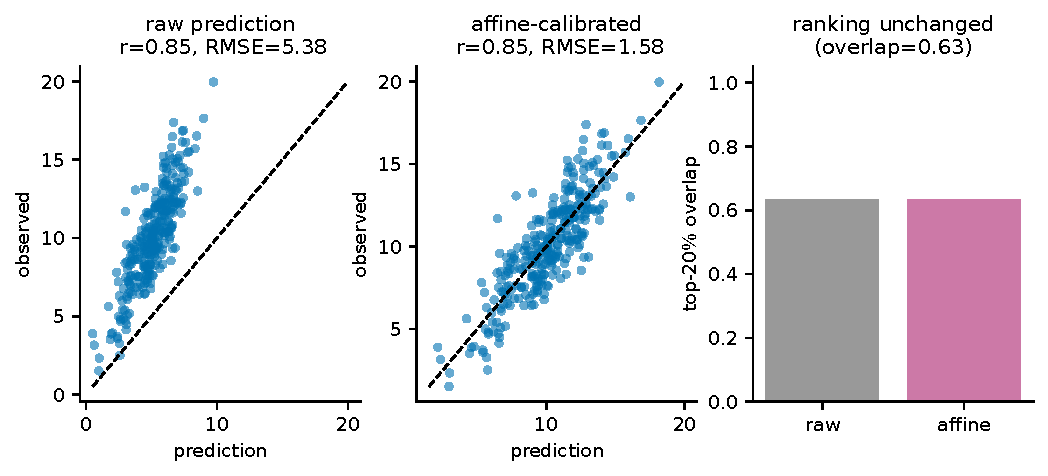
\includegraphics[width=\linewidth]{figures/fig2_simulation.pdf}}{}
\caption{Controlled simulation of Proposition~\ref{prop:2}: a well-correlated but
mis-scaled prediction (left) is corrected by affine calibration (middle) ---
RMSE falls while Pearson $r$ is unchanged --- and the top-$20\%$ selection
overlap is identical before and after (right).}
\label{fig:simulation}
\end{figure}

\subsection{Mini-batch versus global Pearson}\label{sec:prop3}
\begin{proposition}\label{prop:3}
For a partition of the data into batches $B_1,\dots,B_K$, the batch-averaged loss
$\tfrac1K\sum_k \bigl(1-r_{B_k}\bigr)$ is not equal to $1-r_{\mathrm{global}}$ in
general, because $r$ is a non-linear (ratio-of-moments) functional of the data.
Because the functional is nonlinear, neither equality nor a monotonic relation
between batch size and discrepancy is guaranteed without further assumptions.
\end{proposition}
A full-batch evaluation of $\mathcal{L}_{\mathrm{P}}$ optimizes the global
objective exactly; a large batch is an approximation, and smaller batches
optimize a noisier surrogate. A supporting experiment quantifies the practical
effect over the tested range.

\subsection{Multi-trait and group-aware variants}\label{sec:groupaware}
The loss extends naturally to $T$ traits, $\mathcal{L}=\tfrac1T\sum_{t=1}^T
(1-r_t)$ (or a weighted sum $\sum_t w_t(1-r_t)$), and to a group-aware objective
$\mathcal{L}=\tfrac1G\sum_{g=1}^G (1-r_g)$ where $g$ indexes environments, years,
families or sites --- aligning training with the within-environment correlation
that multi-environment breeding programs actually care about. As in
Proposition~\ref{prop:3}, neither variant equals the pooled global correlation.

\section{Materials and Methods}\label{sec:methods}

\paragraph{Datasets.} We use three public sources, for a total of \NUM{101}
trait--dataset combinations across \NUM{12} panels/sources spanning 10 species. (i) \emph{EasyGeSe}
\citep{quesada2025easygese}: a benchmark of ten species (barley, common bean,
lentil, maize, eastern oyster, pig, loblolly pine, rice, soybean and wheat)
providing genotypes, phenotypes and \emph{fixed} cross-validation partitions; the
maize set is the global genotype-by-environment competition panel
\citep{washburn2025maize}. (ii) The CIMMYT \emph{wheat} panel
\citep{crossa2010}: 599 lines, 1{,}279 DArT markers and grain yield in four
environments, analyzed as four outcomes. (iii) \emph{SoyNAM}
\citep{xavier2016soynam}: $\sim$5{,}500 recombinant inbred lines in 40 biparental
families, analyzed for four agronomic traits. Genotypes are coded as allele
dosages; preprocessing (unsupervised, no phenotype) applies a minor-allele
frequency filter ($\geq 0.01$), mean imputation, and a top-variance cap at
20{,}000 markers for the seven panels whose marker count exceeded 20{,}000
(barley, lentil, maize, oyster, pig, rice and soybean).
Table~\ref{tab:datasets} and Figure~\ref{fig:datasets} summarize the data.

\begin{table}[t]\centering
\caption{The 101 trait--dataset combinations across 12 panels/sources (10 species;
10 panels from EasyGeSe, plus CIMMYT wheat and SoyNAM). $n$ is the number of genotypes, $p$ the markers used
(after MAF filtering and the 20{,}000-marker variance cap), and GBLUP $r$ the mean
within-dataset predictive ability of GBLUP (a difficulty index).}\label{tab:datasets}
\begin{tabular}{lrrrrl}
\toprule
Species & $n$ & $p$ & traits & GBLUP $r$ & source\\
\midrule
rice & 352 & 20{,}000 & 36 & 0.46 & EasyGeSe \\
pine & 925 & 4{,}421 & 17 & 0.82 & EasyGeSe \\
wheatG & 371 & 12{,}546 & 16 & 0.59 & EasyGeSe \\
maize & 4421 & 20{,}000 & 6 & 0.83 & EasyGeSe \\
bean & 444 & 16{,}707 & 5 & 0.57 & EasyGeSe \\
lentil & 324 & 20{,}000 & 5 & 0.79 & EasyGeSe \\
soybeanNAM & 5487 & 4{,}401 & 4 & 0.71 & SoyNAM \\
wheat & 599 & 1{,}279 & 4 & 0.46 & BGLR/CIMMYT \\
barley & 1438 & 20{,}000 & 2 & 0.58 & EasyGeSe \\
oyster & 372 & 20{,}000 & 2 & 0.38 & EasyGeSe \\
pig & 1709 & 20{,}000 & 2 & 0.31 & EasyGeSe \\
soybean & 346 & 20{,}000 & 2 & 0.40 & EasyGeSe \\
\bottomrule
\end{tabular}

\vspace{2pt}
{\footnotesize\raggedright The count of 12 panels/sources (spanning 10 species)
treats related germplasm
sharing a common crop as distinct panels: wheatG (EasyGeSe) and wheat (CIMMYT) are
separate sources, as are soybean (EasyGeSe) and soybeanNAM (SoyNAM)
panels of the same species drawn from different sources.\par}
\end{table}

\begin{figure}[tbp]\centering
\IfFileExists{figures/fig3_datasets.pdf}{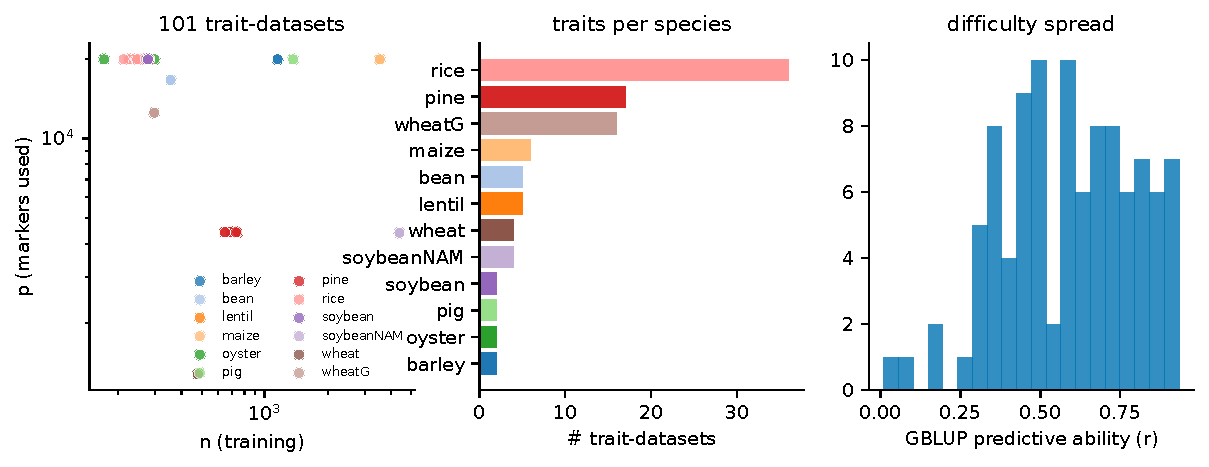
\includegraphics[width=\linewidth]{figures/fig3_datasets.pdf}}{}
\caption{Dataset map: size, dimensionality and predictability across species.}
\label{fig:datasets}
\end{figure}

\paragraph{Models.} The parametric baseline is GBLUP with REML-estimated variance
components, implemented in the spectral basis of the linear genomic kernel
$K=XX^\top/p$ and validated against the \texttt{rrBLUP} package
\citep{endelman2011} to floating-point precision (cross-implementation
correlation $1.0000$). We also include ridge regression as a linear baseline. The neural predictors
are a multilayer perceptron (MLP), a one-dimensional convolutional network over
ordered markers (1D-CNN), a light Transformer over marker patches, and four
protocol-matched, literature-inspired adaptations: DeepGS
\citep{ma2018deepgs}, DNNGP \citep{wang2023dnngp}, PNNGS \citep{pnngs2024}, and
SoyDNGP \citep{gao2023soydngp}. These are not exact reproductions: they retain
published motifs while using common dosage inputs, preprocessing, training and
evaluation. For the primary ablation, one configuration is selected per dataset
registry key and architecture under MSE and frozen across losses. EasyGeSe and
CIMMYT use one representative trait per panel and transfer it to the other
traits; the four SoyNAM phenotypes are separate registry keys and are tuned on
their own phenotype. The contrast changes only the loss conditional on the
configuration, but selection under MSE may favor MSE.

\paragraph{Loss functions.} We compare MSE; the standardized-MSE Pearson loss
$1-r$ (Proposition~\ref{prop:1}); a hybrid $\,(1-r)+\lambda\,\mathrm{MSE}\,$ with
$\lambda=0.1$; and a concordance-correlation loss $1-\rho_c$ \citep{lin1989},
which penalizes correlation, scale and offset jointly. The negative-Pearson and
explicit standardized-MSE forms are included in the numerical checks.

\paragraph{Calibration.} For every model and loss we report predictions under
three post-hoc maps: raw (identity), affine (Proposition~\ref{prop:2}) and
isotonic. Calibrators are fit on validation predictions only.

\paragraph{Cross-validation.} We use the fixed EasyGeSe partitions (5 folds
$\times$ 2 repeats $=$ 10 folds per trait) and repeated $K$-fold for wheat and
SoyNAM. Within each training fold an inner 80/20 split provides early-stopping and
calibration data; markers are standardized with training statistics only;
targets are standardized with training statistics for the neural networks and
predictions are returned in the original units. Neural networks early-stop on the
validation value of the loss being trained. The test fold is never used for
fitting, early stopping or calibration. Primary hyper-parameters, however, were
selected before outer CV on the full tuning phenotype described above, so
absolute performance is not a nested estimate. In a separate CIMMYT sensitivity,
MSE and Pearson each received the same eight-candidate bank inside five outer
folds using only environment-1 outer-training observations; configurations were
evaluated in four environments with three initialization seeds.

\paragraph{Evaluation metrics.} Predictive: Pearson $r$, Spearman $\rho$, RMSE,
MAE, $R^2$, mean bias, and the calibration slope and intercept (ideal $1$ and
$0$). Upper-tail ranking, at intensities $k\in\{5,10,15,20\}\%$: top-$k$ overlap,
precision@$k$, recall@$k$, NDCG@$k$ \citep{jarvelin2002ndcg}, selection
differential, mean phenotype of the selected, and relative efficiency (achieved
upper-tail differential divided by the oracle differential). Larger phenotypes
are always the target; these metrics are not interpreted as breeding gain when
lower or intermediate values are desirable.

\paragraph{Statistical analysis.} For each task, architecture and loss we first
average the ten fold values and form
$\Delta m=m_{\mathrm{loss}}-m_{\mathrm{MSE}}$. The pooled contrast averages the
seven architectures within task. The primary estimand gives equal weight to each
of 12 panels; a trait-weighted estimand is a sensitivity check. Confidence
intervals resample panels as clusters (20,000 replicates), and an exact two-sided
sign-flip test reverses all task contrasts within a panel together.
Leave-one-panel-out ranges assess influence. A corroborative mixed model of the
paired deltas contains loss, architecture, their interaction, panel as a blocking
factor and a random task intercept; a likelihood-ratio test compares models with
and without the interaction. Raw Pearson is the prespecified primary endpoint,
raw NDCG@$10$ is secondary, and RMSE is normalized by the test-fold phenotype
standard deviation after validation-fitted affine calibration. The nested-HPO
experiment covers MLP, CNN and Transformer only and is analyzed separately and descriptively because its environments,
folds and seeds are repeated measures from one wheat panel.

\paragraph{Implementation.} The framework is released as the Python package
\texttt{ccgp}, built on PyTorch \citep{paszke2019pytorch}, scikit-learn
\citep{pedregosa2011sklearn} and NumPy
\citep{harris2020numpy}, with the neural networks trained using the Adam optimizer
\citep{kingma2015adam}, deterministic split definitions and recorded tuned
configurations. The main campaign used one initialization per fold; only the
nested wheat sensitivity used three seeds. Analysis scripts validate the
90,900-row campaign and 1,080-row nested result files before producing tables
and machine-readable figure source data.

\input{sec_results.tex}

\input{discussion_body.tex}

\section{Conclusion}
A standardized-MSE Pearson loss aligns neural-network training with the
predictive-ability metric used throughout genomic prediction; because correlation
is scale-free, a separate calibration step or a scale-aware objective is needed
when calibrated phenotypic values matter; and global correlation should be
complemented by decision-specific metrics. Empirically, across 101 trait--datasets the average
benefit is small, sensitive to panel weighting, and not uniform across
architectures. The clearest descriptive signal occurs for the Transformer,
while DeepGS provides a negative counterexample, and no neural loss unseated
GBLUP or ridge on mean rank. Together, these results provide a practical
framework for separating objective alignment, phenotypic calibration and
decision-level evaluation in neural genomic prediction; Pearson or CCC should be
viewed as objective-specific alternatives to test alongside MSE rather than as
universal replacements.

\section*{Data availability}
All datasets are public: EasyGeSe (Zenodo, DOI \texttt{10.5281/zenodo.15348871}), the CIMMYT wheat panel
(\texttt{BGLR} R package \citep{perez2014bglr}) and SoyNAM (\texttt{SoyNAM} R package). Code, fixed
cross-validation partitions, tuned configurations and a recorded runtime manifest are
released as the \texttt{ccgp} package, with source at
\url{https://github.com/GBeurier/gs-loss} (a versioned archive will be
deposited at Zenodo, DOI to be assigned). All datasets used in the reported
benchmark are public and download automatically. Supporting Information (File~S1,
\texttt{supplement.pdf}) documents the architecture adaptations, complete paired
contrasts, missingness, HPO provenance, calibration, mean ranks and nested wheat
sensitivity. Machine-readable source tables accompany every data-driven figure.

\bibliographystyle{apalike}
\bibliography{refs}



\end{document}
"  for a
% line-numbered bioRxiv preprint; default (0) is the clean submission build.
\providecommand{\PREPRINTMODE}{0}
\ifnum\PREPRINTMODE=1 \usepackage[switch]{lineno}\fi

\theoremstyle{plain}
\newtheorem{proposition}{Proposition}
\theoremstyle{remark}
\newtheorem{remark}{Remark}

\title{\bfseries Metric-consistent neural networks for genomic prediction and
selection: a standardized-MSE Pearson loss, affine calibration, and
selection-aware evaluation}

\author[1,2]{Gr\'egory Beurier\thanks{Corresponding author: \texttt{gregory.beurier@cirad.fr}}}
\author[1,2]{Denis Cornet}
\author[1,2]{Lauriane Rouan}
\author[1,2]{David Cros}
\affil[1]{CIRAD, UMR AGAP Institut, Montpellier, France}
\affil[2]{UMR AGAP Institut, Univ Montpellier, CIRAD, INRAE, Institut Agro, Montpellier, France}
\date{\ifnum\PREPRINTMODE=1 \textit{Preprint --- not peer-reviewed} \quad\textbullet\quad \today\else\today\fi}

\begin{document}
\maketitle
\ifnum\PREPRINTMODE=1 \linenumbers \fi

\begin{abstract}
\noindent
Genomic prediction involves three objectives that are often conflated:
association with phenotype, calibration to the phenotypic scale, and recovery of
selection candidates. Neural predictors are usually trained by mean squared
error (MSE), although predictive ability is commonly evaluated by Pearson
correlation and candidate ranking. We use the identity
$\mathrm{MSE}(z_y,z_{\hat y})=2(1-r)$ to implement a stable differentiable
Pearson objective and ask what is gained, and what is not, by aligning the
training objective with the correlation metric. A shared-configuration ablation compared MSE,
Pearson, hybrid and concordance-correlation losses for seven architectures on
101 public trait--dataset tasks from 12 panels spanning ten species. Folds were
averaged before inference; effects were balanced across panels and uncertainty
was obtained by panel-cluster bootstrap. Relative to MSE, Pearson training gave
a small positive raw-correlation estimate of $0.0048$ (95\% cluster bootstrap
interval $0.0008$--$0.0091$), while an exact 12-panel sign-flip test was just
above the conventional threshold ($p=0.052$). Raw Pearson predictions were
poorly scaled (normalized-RMSE change $+0.346$ relative to raw MSE), but
validation-fitted affine calibration removed this penalty ($-0.0033$) without
materially changing correlation. The corresponding change in NDCG@$10$ was
only $0.0018$ ($-0.0001$--$0.0035$). Estimates varied across architectures: the Transformer had
the clearest positive contrast ($+0.0176$), whereas the DeepGS-inspired network
had a negative contrast ($-0.0067$); the global loss-by-architecture interaction
was inconclusive. A separate loss-specific nested-HPO sensitivity for MLP, CNN
and Transformer on CIMMYT wheat supported a Transformer signal but not a uniform benefit and revealed
material seed variability. Affine calibration restored phenotypic scale, although an
unconstrained negative validation slope occasionally reversed rankings. Thus a
differentiable Pearson loss is feasible, but metric-consistent training is most
useful as part of a workflow in which objective alignment, calibration and
selection performance are evaluated separately rather than as a universal
replacement for MSE.

\end{abstract}

\section{Introduction}

Genomic selection \citep{meuwissen2001} predicts the genetic merit of candidate
individuals from genome-wide markers, and has become central to modern plant and
animal breeding \citep{heffner2009,jannink2010,desta2014}. The dominant
parametric baseline, genomic best linear unbiased prediction
(GBLUP)/ridge-regression BLUP \citep{vanraden2008,endelman2011}, is increasingly
complemented by machine-learning and deep-learning predictors
\citep{ma2018deepgs,wang2023dnngp,montesinos2021review,montesinos2021power}.
Whether deep learning improves on GBLUP remains dataset-dependent: recent
comparisons find that neither systematically dominates, and that outcomes hinge
on tuning, architecture and the choice of evaluation metric
\citep{montesinos2025dlgblup}.

That last point is the subject of this paper. Genomic predictors are trained, by
near-universal default, to minimize the mean squared error (MSE). But they are
\emph{assessed} with the Pearson correlation $r$ between predicted and observed
phenotypes --- the ``predictive ability'' reported in essentially every genomic
prediction study \citep{crossa2010} --- and they are \emph{used} to rank
candidates and select the best ones. There is therefore a systematic mismatch
between the training objective and one of the principal metrics used to evaluate
genomic prediction. More importantly, neither MSE nor Pearson correlation is
identical to the ranking problem ultimately faced in selection.
\citet{waldmann2019} showed that selecting a model by $r$ can disagree with
selecting it by MSE or $R^2$. \citet{ornella2014} argued that $r$ is a poor guide
to performance in the tails of the distribution, where selection actually
operates, and evaluated the recovery of the best $\alpha\in\{10,\dots,40\}\%$ of
individuals. \citet{blondel2015} reframed genomic selection as a ranking problem,
introduced NDCG from information retrieval as an accuracy measure, and reported
that $r$ correlates poorly with ranking quality.

If correlation is the target, why not train for it directly? A recent
convolutional architecture for genomic selection states plainly that ``Pearson
correlation cannot be set as the loss function'' and substitutes a family of
$L_p$ losses \citep{pnngs2024}. We show this premise is false. The Pearson
correlation \emph{is} a loss --- a standardized MSE --- and training with it is
both well posed and numerically stable. The remaining objection to a correlation
loss, that it ignores scale and offset, is real but easily and provably remedied
by an affine recalibration applied after training.

The empirical question therefore has a simple three-stage structure: compare
the usual MSE-trained raw predictions with Pearson-trained raw predictions to
measure correlation alignment, then calibrate the Pearson outputs on validation
data to recover phenotypic scale, and finally evaluate separately whether
correlation-aligned training changes upper-tail selection. Figure~\ref{fig:loss}
carries this structure through to the headline result.

\paragraph{Contributions.}
\begin{enumerate}
\item \textbf{A standardized-MSE Pearson loss (Section~\ref{sec:prop1}).} We give
the exact identity $\mathrm{MSE}(z_y,z_{\hat y}) = 2(1-r)$ and use it as a stable,
differentiable training objective, verified numerically (to single-precision
tolerance for the loss; to float64 machine precision for the calibration identity).
\item \textbf{Affine calibration with a closed form
(Section~\ref{sec:prop2}).} We prove that the optimal post-hoc affine map yields
residual error $\sigma_y^2(1-r^2)$ on the fitting sample and restores scale and
offset while preserving $r$ and rankings whenever the fitted slope is positive.
\item \textbf{Mini-batch analysis (Section~\ref{sec:prop3}).} We show the
mini-batch Pearson loss is a biased surrogate for the global objective and
quantify the effect of batch size empirically.
\item \textbf{A reproducible, selection-aware benchmark
(Sections~\ref{sec:methods}--\ref{sec:results}).} Across \NUM{101}
trait--datasets from \NUM{12} panels/sources spanning 10 species, with architecture, splits and tuning held
fixed so that only the loss changes, we report both predictive and
selection-oriented metrics, a confirmatory mixed-model analysis, and a
meta-analysis of \emph{when} correlation-consistent training helps. All data are
public and all code, splits and tuned configurations are released.
\end{enumerate}

\noindent We do not claim that a Pearson loss is uniformly superior to MSE; that
would be false. We provide a principled, reproducible framework for training,
calibrating and evaluating neural genomic predictors by treating predictive correlation,
phenotypic scale and selection as related but distinct objectives.

\section{Theory}\label{sec:theory}
Throughout, $y,\hat y\in\mathbb{R}^n$, with sample means $\bar y,\bar{\hat y}$ and
population variances $\sigma_x^2 = \tfrac1n\sum_i (x_i-\bar x)^2$. The Pearson
correlation is $r=r(y,\hat y)=\tfrac1n\sum_i z_{y,i} z_{\hat y,i}$ where
$z_{x,i}=(x_i-\bar x)/\sigma_x$ is the standardized variable.

\subsection{The Pearson loss is a standardized MSE}\label{sec:prop1}
\begin{proposition}\label{prop:1}
For non-degenerate $y,\hat y$ (i.e.\ $\sigma_y,\sigma_{\hat y}>0$),
\[
\mathrm{MSE}(z_y,z_{\hat y}) \;=\; \tfrac1n\sum_{i=1}^n (z_{y,i}-z_{\hat y,i})^2
\;=\; 2\,(1-r).
\]
Consequently $1-r = \tfrac12\,\mathrm{MSE}(z_y,z_{\hat y})$, and minimizing the
standardized MSE is exactly maximizing the Pearson correlation.
\end{proposition}
\begin{proof}
Expanding the square,
$\tfrac1n\sum_i (z_{y,i}-z_{\hat y,i})^2
= \tfrac1n\sum_i z_{y,i}^2 - 2\tfrac1n\sum_i z_{y,i} z_{\hat y,i}
+ \tfrac1n\sum_i z_{\hat y,i}^2 = 1 - 2r + 1 = 2(1-r)$,
because $\tfrac1n\sum_i z_{x,i}^2 = 1$ by construction and
$\tfrac1n\sum_i z_{y,i} z_{\hat y,i}=r$.
\end{proof}
This gives the loss $\mathcal{L}_{\mathrm{P}}(\hat y,y) = 1-r(\hat y,y)$,
implemented directly with a small $\varepsilon$ guarding the standard-deviation
denominators and numerically equivalent to
$\tfrac12\,\mathrm{MSE}(z_y,z_{\hat y})$. It is differentiable everywhere
$\sigma_{\hat y}>0$; we verify the gradient against finite differences and verify
the identity to single-precision tolerance in Section~\ref{sec:res-numerical}. The
negative-correlation loss $-r$ differs from $\mathcal{L}_{\mathrm{P}}$ by a
constant and has identical gradients.

\begin{figure}[tbp]\centering
\IfFileExists{figures/fig1_geometry.pdf}{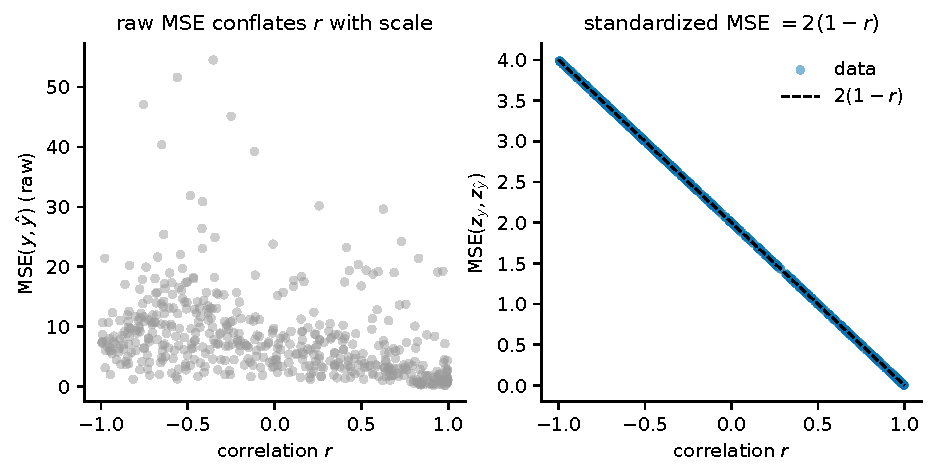
\includegraphics[width=\linewidth]{figures/fig1_geometry.pdf}}{}
\caption{Geometry of the standardized-MSE / Pearson identity (Proposition~\ref{prop:1}).}
\label{fig:geometry}
\end{figure}

\subsection{Affine calibration restores scale without changing rank}\label{sec:prop2}
Correlation is invariant to strictly increasing affine transformations of $\hat
y$: a model trained on $\mathcal{L}_{\mathrm{P}}$ controls the \emph{shape} of the
prediction but not its scale or offset. This is corrected exactly and cheaply.
\begin{proposition}\label{prop:2}
Let $p\in\mathbb{R}^n$ be raw predictions and $r=r(y,p)$. The affine map
$\tilde y = a\,p+b$ minimizing $\tfrac1n\sum_i (a p_i + b - y_i)^2$ has
\[
a^\star = \frac{\mathrm{cov}(y,p)}{\mathrm{var}(p)},\qquad
b^\star = \bar y - a^\star\,\bar p,\qquad
\mathrm{MSE}_{\min} = \sigma_y^2\,(1-r^2).
\]
If $a^\star>0$, the map is strictly increasing and hence preserves $r$, the
Spearman correlation, and every top-$k$/ranking quantity, while setting the
calibration slope to $1$ and intercept to $0$.
\end{proposition}
\begin{proof}
Ordinary least squares for a single predictor gives $a^\star,b^\star$ as stated;
the minimized residual variance of simple linear regression is
$\sigma_y^2(1-r^2)$. A strictly increasing transform preserves the order of $p$
and leaves correlation-type and rank-based statistics unchanged.
\end{proof}
We fit $(a^\star,b^\star)$ on held-out validation predictions (never on the test
set) and apply them to the test predictions. Isotonic regression provides a
monotone non-linear alternative when the raw-vs-true relationship is monotone but
curved. A positive affine map preserves $r$; a negative affine slope changes its
sign, and nonlinear isotonic calibration can change its magnitude. Calibration
can nonetheless improve RMSE, bias and slope (Figure~\ref{fig:simulation};
Section~\ref{sec:res-calibration}).

\begin{figure}[tbp]\centering
\IfFileExists{figures/fig2_simulation.pdf}{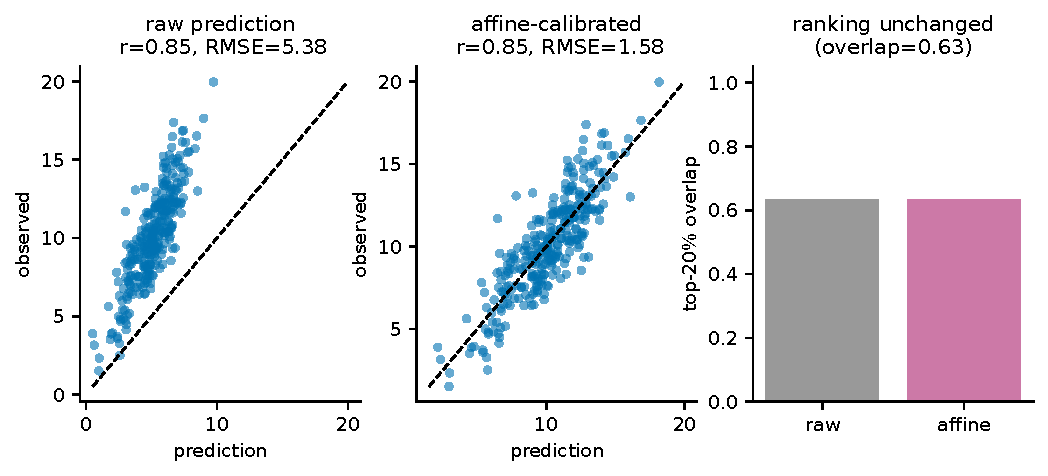
\includegraphics[width=\linewidth]{figures/fig2_simulation.pdf}}{}
\caption{Controlled simulation of Proposition~\ref{prop:2}: a well-correlated but
mis-scaled prediction (left) is corrected by affine calibration (middle) ---
RMSE falls while Pearson $r$ is unchanged --- and the top-$20\%$ selection
overlap is identical before and after (right).}
\label{fig:simulation}
\end{figure}

\subsection{Mini-batch versus global Pearson}\label{sec:prop3}
\begin{proposition}\label{prop:3}
For a partition of the data into batches $B_1,\dots,B_K$, the batch-averaged loss
$\tfrac1K\sum_k \bigl(1-r_{B_k}\bigr)$ is not equal to $1-r_{\mathrm{global}}$ in
general, because $r$ is a non-linear (ratio-of-moments) functional of the data.
Because the functional is nonlinear, neither equality nor a monotonic relation
between batch size and discrepancy is guaranteed without further assumptions.
\end{proposition}
A full-batch evaluation of $\mathcal{L}_{\mathrm{P}}$ optimizes the global
objective exactly; a large batch is an approximation, and smaller batches
optimize a noisier surrogate. A supporting experiment quantifies the practical
effect over the tested range.

\subsection{Multi-trait and group-aware variants}\label{sec:groupaware}
The loss extends naturally to $T$ traits, $\mathcal{L}=\tfrac1T\sum_{t=1}^T
(1-r_t)$ (or a weighted sum $\sum_t w_t(1-r_t)$), and to a group-aware objective
$\mathcal{L}=\tfrac1G\sum_{g=1}^G (1-r_g)$ where $g$ indexes environments, years,
families or sites --- aligning training with the within-environment correlation
that multi-environment breeding programs actually care about. As in
Proposition~\ref{prop:3}, neither variant equals the pooled global correlation.

\section{Materials and Methods}\label{sec:methods}

\paragraph{Datasets.} We use three public sources, for a total of \NUM{101}
trait--dataset combinations across \NUM{12} panels/sources spanning 10 species. (i) \emph{EasyGeSe}
\citep{quesada2025easygese}: a benchmark of ten species (barley, common bean,
lentil, maize, eastern oyster, pig, loblolly pine, rice, soybean and wheat)
providing genotypes, phenotypes and \emph{fixed} cross-validation partitions; the
maize set is the global genotype-by-environment competition panel
\citep{washburn2025maize}. (ii) The CIMMYT \emph{wheat} panel
\citep{crossa2010}: 599 lines, 1{,}279 DArT markers and grain yield in four
environments, analyzed as four outcomes. (iii) \emph{SoyNAM}
\citep{xavier2016soynam}: $\sim$5{,}500 recombinant inbred lines in 40 biparental
families, analyzed for four agronomic traits. Genotypes are coded as allele
dosages; preprocessing (unsupervised, no phenotype) applies a minor-allele
frequency filter ($\geq 0.01$), mean imputation, and a top-variance cap at
20{,}000 markers for the seven panels whose marker count exceeded 20{,}000
(barley, lentil, maize, oyster, pig, rice and soybean).
Table~\ref{tab:datasets} and Figure~\ref{fig:datasets} summarize the data.

\begin{table}[t]\centering
\caption{The 101 trait--dataset combinations across 12 panels/sources (10 species;
10 panels from EasyGeSe, plus CIMMYT wheat and SoyNAM). $n$ is the number of genotypes, $p$ the markers used
(after MAF filtering and the 20{,}000-marker variance cap), and GBLUP $r$ the mean
within-dataset predictive ability of GBLUP (a difficulty index).}\label{tab:datasets}
\begin{tabular}{lrrrrl}
\toprule
Species & $n$ & $p$ & traits & GBLUP $r$ & source\\
\midrule
rice & 352 & 20{,}000 & 36 & 0.46 & EasyGeSe \\
pine & 925 & 4{,}421 & 17 & 0.82 & EasyGeSe \\
wheatG & 371 & 12{,}546 & 16 & 0.59 & EasyGeSe \\
maize & 4421 & 20{,}000 & 6 & 0.83 & EasyGeSe \\
bean & 444 & 16{,}707 & 5 & 0.57 & EasyGeSe \\
lentil & 324 & 20{,}000 & 5 & 0.79 & EasyGeSe \\
soybeanNAM & 5487 & 4{,}401 & 4 & 0.71 & SoyNAM \\
wheat & 599 & 1{,}279 & 4 & 0.46 & BGLR/CIMMYT \\
barley & 1438 & 20{,}000 & 2 & 0.58 & EasyGeSe \\
oyster & 372 & 20{,}000 & 2 & 0.38 & EasyGeSe \\
pig & 1709 & 20{,}000 & 2 & 0.31 & EasyGeSe \\
soybean & 346 & 20{,}000 & 2 & 0.40 & EasyGeSe \\
\bottomrule
\end{tabular}

\vspace{2pt}
{\footnotesize\raggedright The count of 12 panels/sources (spanning 10 species)
treats related germplasm
sharing a common crop as distinct panels: wheatG (EasyGeSe) and wheat (CIMMYT) are
separate sources, as are soybean (EasyGeSe) and soybeanNAM (SoyNAM)
panels of the same species drawn from different sources.\par}
\end{table}

\begin{figure}[tbp]\centering
\IfFileExists{figures/fig3_datasets.pdf}{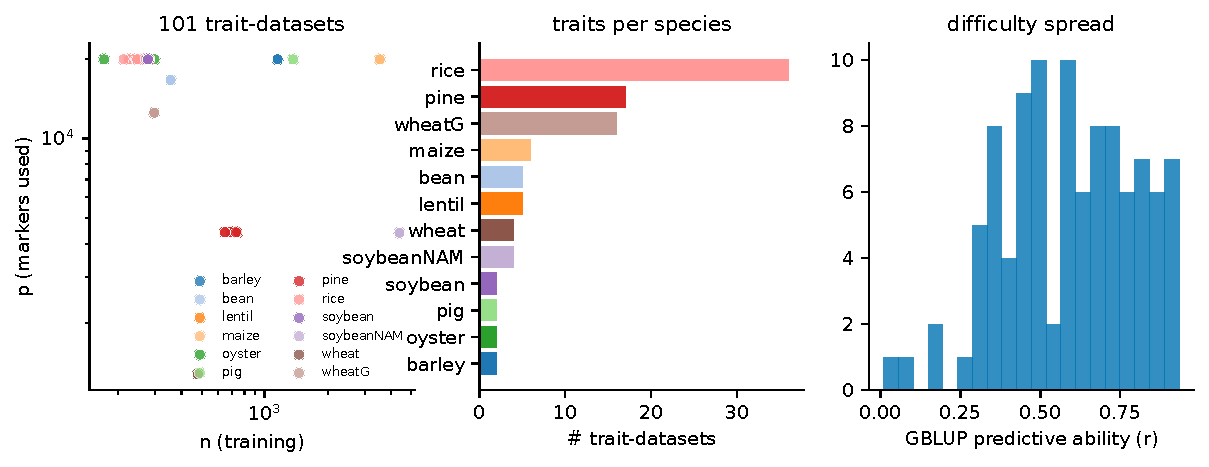
\includegraphics[width=\linewidth]{figures/fig3_datasets.pdf}}{}
\caption{Dataset map: size, dimensionality and predictability across species.}
\label{fig:datasets}
\end{figure}

\paragraph{Models.} The parametric baseline is GBLUP with REML-estimated variance
components, implemented in the spectral basis of the linear genomic kernel
$K=XX^\top/p$ and validated against the \texttt{rrBLUP} package
\citep{endelman2011} to floating-point precision (cross-implementation
correlation $1.0000$). We also include ridge regression as a linear baseline. The neural predictors
are a multilayer perceptron (MLP), a one-dimensional convolutional network over
ordered markers (1D-CNN), a light Transformer over marker patches, and four
protocol-matched, literature-inspired adaptations: DeepGS
\citep{ma2018deepgs}, DNNGP \citep{wang2023dnngp}, PNNGS \citep{pnngs2024}, and
SoyDNGP \citep{gao2023soydngp}. These are not exact reproductions: they retain
published motifs while using common dosage inputs, preprocessing, training and
evaluation. For the primary ablation, one configuration is selected per dataset
registry key and architecture under MSE and frozen across losses. EasyGeSe and
CIMMYT use one representative trait per panel and transfer it to the other
traits; the four SoyNAM phenotypes are separate registry keys and are tuned on
their own phenotype. The contrast changes only the loss conditional on the
configuration, but selection under MSE may favor MSE.

\paragraph{Loss functions.} We compare MSE; the standardized-MSE Pearson loss
$1-r$ (Proposition~\ref{prop:1}); a hybrid $\,(1-r)+\lambda\,\mathrm{MSE}\,$ with
$\lambda=0.1$; and a concordance-correlation loss $1-\rho_c$ \citep{lin1989},
which penalizes correlation, scale and offset jointly. The negative-Pearson and
explicit standardized-MSE forms are included in the numerical checks.

\paragraph{Calibration.} For every model and loss we report predictions under
three post-hoc maps: raw (identity), affine (Proposition~\ref{prop:2}) and
isotonic. Calibrators are fit on validation predictions only.

\paragraph{Cross-validation.} We use the fixed EasyGeSe partitions (5 folds
$\times$ 2 repeats $=$ 10 folds per trait) and repeated $K$-fold for wheat and
SoyNAM. Within each training fold an inner 80/20 split provides early-stopping and
calibration data; markers are standardized with training statistics only;
targets are standardized with training statistics for the neural networks and
predictions are returned in the original units. Neural networks early-stop on the
validation value of the loss being trained. The test fold is never used for
fitting, early stopping or calibration. Primary hyper-parameters, however, were
selected before outer CV on the full tuning phenotype described above, so
absolute performance is not a nested estimate. In a separate CIMMYT sensitivity,
MSE and Pearson each received the same eight-candidate bank inside five outer
folds using only environment-1 outer-training observations; configurations were
evaluated in four environments with three initialization seeds.

\paragraph{Evaluation metrics.} Predictive: Pearson $r$, Spearman $\rho$, RMSE,
MAE, $R^2$, mean bias, and the calibration slope and intercept (ideal $1$ and
$0$). Upper-tail ranking, at intensities $k\in\{5,10,15,20\}\%$: top-$k$ overlap,
precision@$k$, recall@$k$, NDCG@$k$ \citep{jarvelin2002ndcg}, selection
differential, mean phenotype of the selected, and relative efficiency (achieved
upper-tail differential divided by the oracle differential). Larger phenotypes
are always the target; these metrics are not interpreted as breeding gain when
lower or intermediate values are desirable.

\paragraph{Statistical analysis.} For each task, architecture and loss we first
average the ten fold values and form
$\Delta m=m_{\mathrm{loss}}-m_{\mathrm{MSE}}$. The pooled contrast averages the
seven architectures within task. The primary estimand gives equal weight to each
of 12 panels; a trait-weighted estimand is a sensitivity check. Confidence
intervals resample panels as clusters (20,000 replicates), and an exact two-sided
sign-flip test reverses all task contrasts within a panel together.
Leave-one-panel-out ranges assess influence. A corroborative mixed model of the
paired deltas contains loss, architecture, their interaction, panel as a blocking
factor and a random task intercept; a likelihood-ratio test compares models with
and without the interaction. Raw Pearson is the prespecified primary endpoint,
raw NDCG@$10$ is secondary, and RMSE is normalized by the test-fold phenotype
standard deviation after validation-fitted affine calibration. The nested-HPO
experiment covers MLP, CNN and Transformer only and is analyzed separately and descriptively because its environments,
folds and seeds are repeated measures from one wheat panel.

\paragraph{Implementation.} The framework is released as the Python package
\texttt{ccgp}, built on PyTorch \citep{paszke2019pytorch}, scikit-learn
\citep{pedregosa2011sklearn} and NumPy
\citep{harris2020numpy}, with the neural networks trained using the Adam optimizer
\citep{kingma2015adam}, deterministic split definitions and recorded tuned
configurations. The main campaign used one initialization per fold; only the
nested wheat sensitivity used three seeds. Analysis scripts validate the
90,900-row campaign and 1,080-row nested result files before producing tables
and machine-readable figure source data.

\section{Results}\label{sec:results}

\subsection{Numerical validation}\label{sec:res-numerical}
Across 80 simulated cases, the implemented Pearson loss, $1-r$, and one half of
the standardized MSE agreed to a maximum absolute difference of
$5.0\times10^{-8}$ (mean $7.4\times10^{-9}$). The affine residual identity in
Proposition~\ref{prop:2} agreed to $1.2\times10^{-15}$ over 200 cases. Both the
Pearson and concordance losses passed automatic gradient checks, and $-r$ and
$1-r$ had identical gradients. These checks establish numerical equivalence,
not empirical superiority.

\subsection{Headline result: correlation, calibration and selection separate}\label{sec:res-loss}

\ifdefined\GTHREE\else
\begin{figure}[tbp]\centering
\IfFileExists{figures/fig4_loss_comparison.pdf}{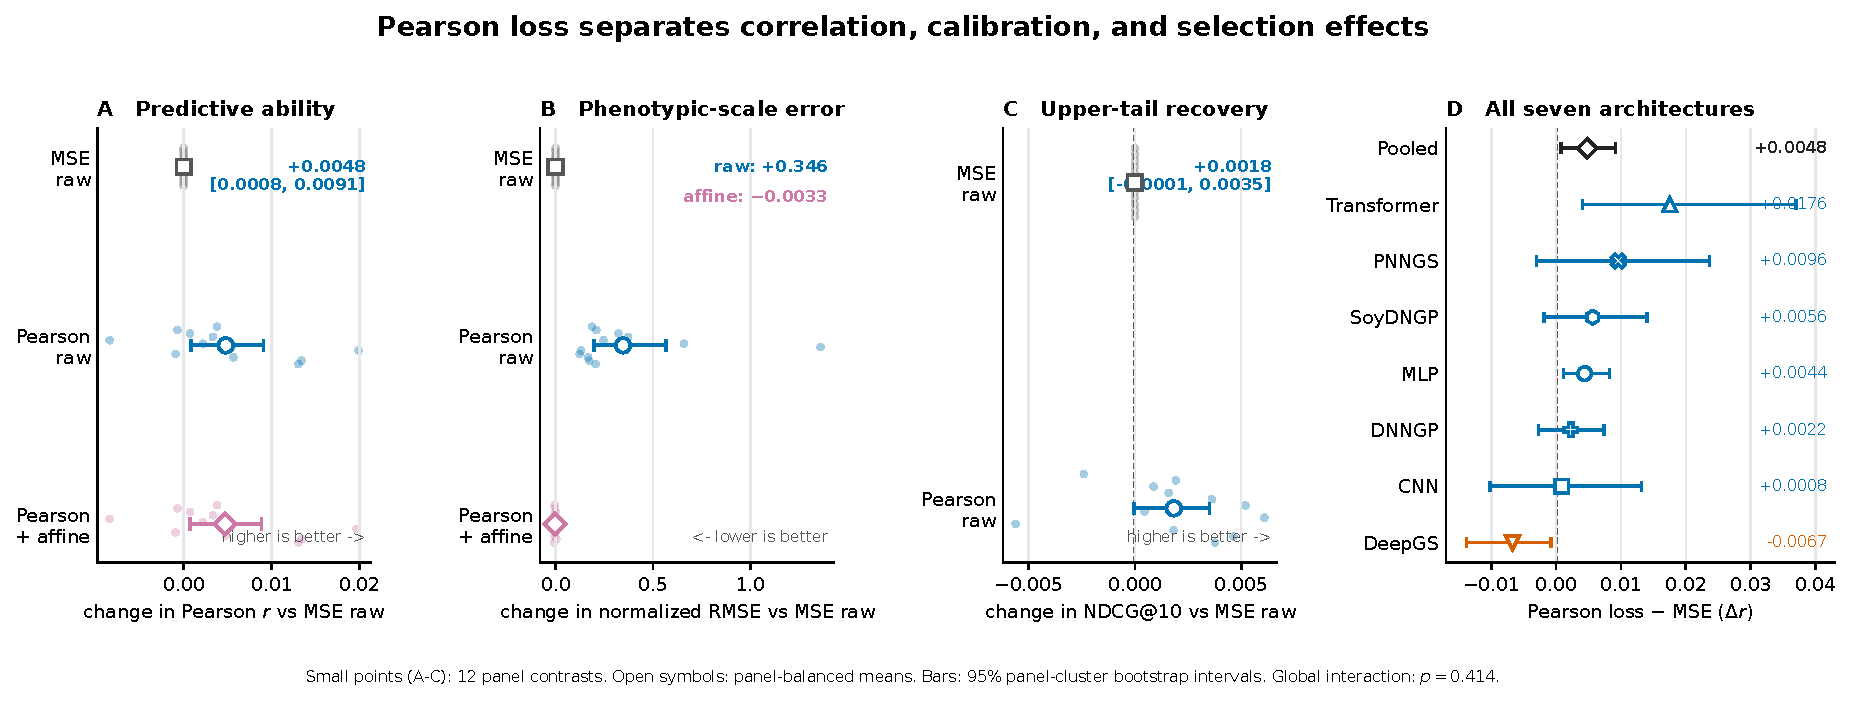
\includegraphics[width=\linewidth]{figures/fig4_loss_comparison.pdf}}{}
\caption{The paper's central comparison. Panels A--B compare the scale-aware
raw MSE baseline, the correlation-targeted but unscaled raw Pearson output, and
the validation-fitted affine Pearson output; Panel C compares raw MSE and raw
Pearson predictions for upper-tail recovery. Small points are contrasts for
each of 12 panels, open symbols are panel-balanced means, and bars are 95\%
panel-cluster bootstrap intervals. Raw Pearson predictions gain $0.0048$ in $r$
but lose $0.346$ in normalized RMSE; affine calibration retains a $0.0047$
correlation gain and changes normalized RMSE by $-0.0033$. The raw NDCG@$10$
change is only $+0.0018$. Panel D reports the Pearson-minus-MSE correlation
contrast, interval and exact point estimate for
the pooled result and every neural architecture in the main benchmark. Folds
were averaged within 101 tasks and architectures within task before panels were
weighted equally.}
\label{fig:loss}
\end{figure}
\fi

Figure~\ref{fig:loss} summarizes the practical sequence. Relative to the
MSE-trained raw baseline, Pearson-trained raw predictions gained $0.0048$ in
correlation but increased normalized RMSE by $0.346$ (95\% panel-cluster
bootstrap interval $[0.1965,0.5675]$), because correlation training does not
identify scale or offset. Validation-fitted affine calibration retained nearly
all of the correlation gain ($+0.0047$) and brought normalized RMSE back to the
MSE baseline ($-0.0033$, $[-0.0062,0.0000]$). Thus the headline is not that
Pearson replaces MSE on every criterion: it slightly improves the target
correlation, a separate calibration step is needed for phenotypic-scale
predictions, and the decision-level effect must be checked directly.

The final grid contained 90,900 rows: seven neural architectures, four losses,
101 tasks, ten test folds and three calibration maps, plus GBLUP and ridge
baselines. All architectures covered the same 101 tasks. After folds were
averaged, the panel-balanced Pearson-minus-MSE contrast for raw test correlation
was $\Delta r=+0.0048$ (95\% panel-cluster bootstrap interval
$[0.0008,0.0091]$). Seventy-eight of 101 task-level pooled
contrasts were positive. An exact test that flipped the signs of all tasks
within each panel gave $p=0.052$, appropriately reflecting that only 12 panels,
not 707 independent experiments, were observed. Weighting every trait equally
instead produced $+0.0101$ ($[0.0028,0.0158]$), showing that the estimate is
sensitive to the many traits contributed by rice, pine and wheatG.

The hybrid and CCC losses gave panel-balanced $\Delta r$ values of $+0.0055$
($[0.0010,0.0100]$) and $+0.0078$ ($[0.0022,0.0139]$), respectively. Figure~\ref{fig:loss}D
reports all seven architecture-specific Pearson contrasts and intervals. The
Transformer has the largest positive estimate ($+0.0176$), while DeepGS is a
negative counterexample ($-0.0067$); PNNGS and SoyDNGP are positive but
uncertain, MLP shows a smaller positive estimate, and DNNGP and CNN lie near
zero. The apparent spread is descriptive: the global loss-by-architecture test
is inconclusive ($\chi^2_{12}=12.40$, $p=0.414$). The four named networks are
literature-inspired adaptations, not exact reproductions of the published systems.

\subsection{Ranking and scale}\label{sec:res-selection}
Pearson training changed panel-balanced raw NDCG@$10$ by only $+0.0018$
($[-0.0001,0.0035]$) and upper-tail overlap by $+0.0033$
($[-0.0010,0.0069]$). CCC gave the largest, still small, NDCG contrast
($+0.0034$, $[0.0015,0.0056]$). These quantities recover the highest observed
phenotypes; because trait desirability was not harmonized, they must not be read
as realized breeding gain for traits where lower values are preferred. Ridge
and GBLUP retained the best mean ranks for both Pearson and NDCG@$10$. The weak
ranking response is therefore an empirical result in its own right: a measurable
gain in global predictive ability did not substantially change which candidates
would be recovered by the upper-tail rule used here.

Affine-calibrated NRMSE, defined as RMSE divided by the test-fold phenotype
standard deviation, was essentially unchanged by Pearson training
($-0.0011$, $[-0.0036,0.0015]$) or the hybrid loss ($-0.0018$,
$[-0.0041,0.0006]$). CCC produced $-0.0028$ ($[-0.0054,-0.0003]$), a very small
normalized-error reduction. Absolute RMSE values were not pooled across traits
because their measurement units differ.

\subsection{Calibration}\label{sec:res-calibration}

\ifdefined\GTHREE\else
\begin{figure}[tbp]\centering
\IfFileExists{figures/fig5_calibration.pdf}{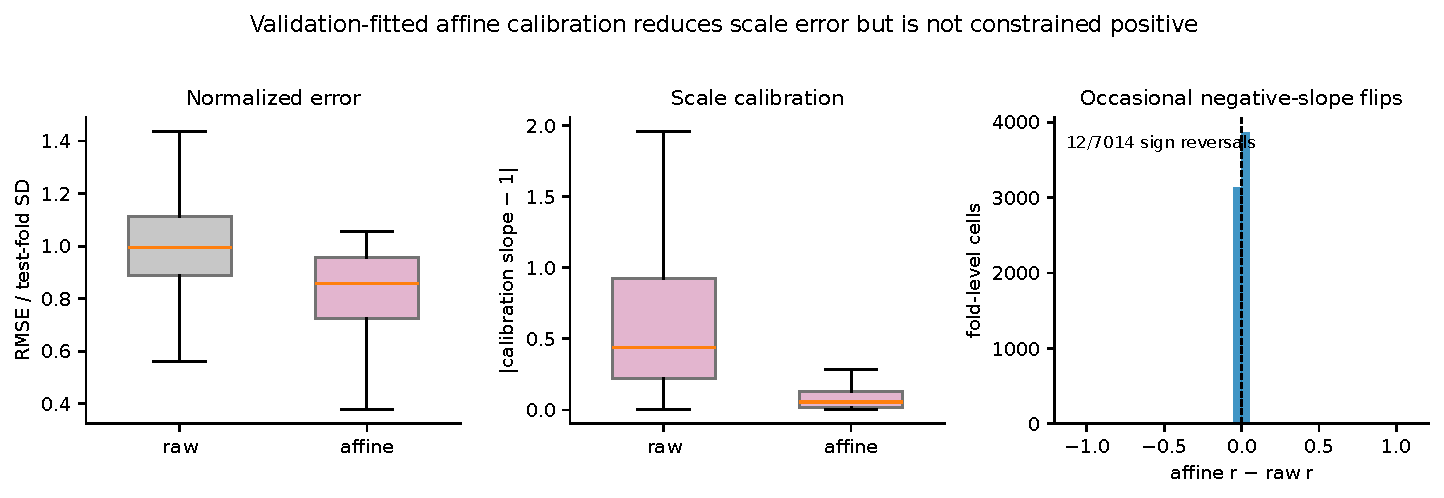
\includegraphics[width=\linewidth]{figures/fig5_calibration.pdf}}{}
\caption{Validation-fitted affine calibration for Pearson-trained networks.
Boxplots summarize 707 task--architecture means (outliers omitted visually);
the histogram uses 7,014 fold-level cells with finite raw and affine
correlations. Calibration reduced normalized error and slope deviation, but 12
folds (0.17\%) had a validation-fitted negative slope that reversed the sign of
test-set correlation.}
\label{fig:calibration}
\end{figure}
\fi

Across Pearson-trained networks, mean RMSE fell from 10.54 to 7.99 after affine
calibration and the median calibration slope moved from 0.918 to 0.957. These
raw-unit averages are descriptive only. A positive affine map preserves ranks,
but the implementation used the unconstrained least-squares slope estimated on
validation data. Among 7,014 comparable fold cells, 12 (0.17\%) therefore
reversed the sign of test correlation. Loss comparisons for correlation and upper-tail recovery use raw predictions.
Figure~\ref{fig:loss} additionally audits raw versus affine correlation to check
that calibration retains the gain. Scale outcomes use affine predictions.

\subsection{Loss-specific HPO and seed sensitivity}\label{sec:res-nested}

\ifdefined\GTHREE\else
\begin{figure}[tbp]\centering
\IfFileExists{figures/fig6_meta.pdf}{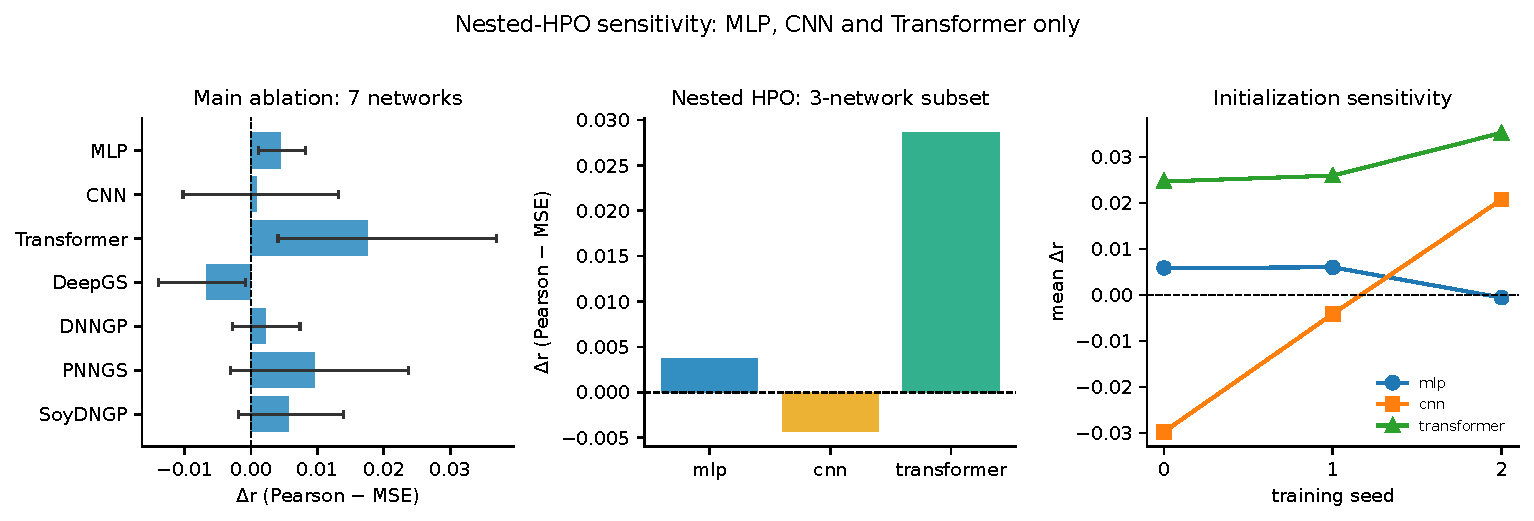
\includegraphics[width=\linewidth]{figures/fig6_meta.pdf}}{}
\caption{Sensitivity to tuning and initialization. The shared-HPO panel shows
panel-balanced effects for all seven networks in the 101-task benchmark. The
nested-HPO and seed panels contain only MLP, CNN and Transformer because
loss-specific nested tuning was run only for these three generic architectures;
the four literature-inspired networks were not evaluated in this sensitivity.
Nested means cover four CIMMYT wheat environments, five outer folds and three
seeds; configurations were selected separately for MSE and Pearson using only
environment-1 observations in each outer-training set. The repeated wheat
outcomes are not independent replications and no confirmatory $p$-value is assigned.}
\label{fig:meta}
\end{figure}
\fi

The nested sensitivity contained 1,080 prediction rows. It was run only for
MLP, CNN and Transformer; DeepGS, DNNGP, PNNGS and SoyDNGP therefore have no
loss-specific nested-HPO result, rather than an omitted result (Figure~\ref{fig:meta}).
Across the three tested architectures, loss-specific Pearson tuning changed raw $r$ by $+0.0093$ on
average. Estimates were $+0.0286$ for the Transformer, $+0.0038$ for the MLP,
and $-0.0044$ for the CNN. Corresponding NDCG@$10$ contrasts were $+0.0069$,
$+0.0071$, and $-0.0060$. CNN's mean $\Delta r$ moved from $-0.0297$ to
$-0.0041$ to $+0.0207$ across seeds 0--2; Transformer remained positive
($+0.0246$, $+0.0259$, $+0.0352$). Thus objective-specific tuning supports the
Transformer signal but also demonstrates initialization uncertainty that the
single-seed main campaign cannot quantify.


\section{Discussion}\label{sec:discussion}

\subsection{A valid objective with a modest empirical effect}
The algebraic result is exact: minimizing standardized MSE maximizes Pearson
correlation. The empirical result is more restrained. Once all seven networks
are evaluated on the same 101 tasks and panels are equally weighted, Pearson
training improves $r$ by about five thousandths. The cluster-bootstrap interval
is positive, but an exact 12-panel sign-flip test lies at the conventional
threshold. The raw Pearson outputs pay a large scale penalty; validation-fitted
affine calibration removes it while leaving the correlation gain essentially
intact. NDCG changes are smaller still. This sequence---align the objective,
then restore scale---and the distinction between mathematical alignment and
modest practical gain are the paper's main findings.

Trait weighting matters. A trait-weighted analysis gives twice the
panel-balanced effect because rice, pine and wheatG contribute many phenotypes.
Neither estimand is intrinsically wrong: the first describes an average listed
trait and the second an average panel. We use panel balance for the headline to
avoid allowing heavily phenotyped resources to determine a cross-panel claim,
and report both for transparency.

\subsection{Architecture heterogeneity is suggestive, not universal}
The Transformer repeatedly shows the largest positive estimate, including after
loss-specific nested tuning. MLP gains are small, CNN is near zero after panel
balance, and the DeepGS-inspired network becomes worse under Pearson training.
This counterexample rules out a universal optimization advantage. At the same
time, the omnibus loss-by-architecture interaction is not significant, so the
apparent ordering should be treated as hypothesis-generating rather than as a
formal taxonomy of networks. Possible mechanisms include different curvature,
normalization and early-stopping behavior, but the present benchmark does not
identify them.

The four named systems are protocol-matched, literature-inspired adaptations.
DeepGS retains a marker convolution/dense motif but adds batch normalization;
DNNGP is genotype-only and uses PCA rather than reproducing its complete
multi-omic setting; PNNGS retains parallel residual kernels but changes the
stem, pooling and validation protocol; and SoyDNGP converts dosage vectors to a
96$\times$96 one-channel representation rather than the published
206$\times$206$\times$3 encoding. Their results evaluate whether these motifs
respond to the loss under one common protocol, not whether the original papers
would reproduce identically.

\subsection{Correlation, calibration and upper-tail recovery}
Correlation is invariant to positive affine transformations, making scale
calibration a separate problem. Validation-fitted affine calibration reduced
normalized error in aggregate, but unconstrained least squares occasionally
estimated a negative slope and reversed rankings. A production implementation
should constrain the slope to be positive or fall back to an intercept-only
map. We avoided this ambiguity by using raw outputs for correlation and ranking
and affine outputs only for scale outcomes.

The upper-tail metrics answer a narrower question than biological selection.
They quantify recovery of the largest observed phenotypes. Some disease,
maturity and moisture traits favor lower or intermediate values, and the public
metadata did not provide a uniform desirability direction. Consequently these
metrics cannot establish breeding utility without trait-specific economic
weights and target directions. Their weak improvement nevertheless shows that a
small gain in global correlation need not translate into a substantial change
in the selected set, consistent with earlier ranking-based critiques
\citep{ornella2014,blondel2015}.

\subsection{What the HPO comparison does and does not show}
The main experiment is a controlled shared-configuration ablation. For each
panel and architecture, a configuration selected under MSE on one representative
trait was transferred to all traits and frozen across losses. This isolates the
training objective conditional on that configuration, but it can favor MSE and
uses the tuning phenotype before outer evaluation; it is not nested
performance estimation. The separate CIMMYT experiment selects MSE and Pearson
configurations inside each outer-training set from identical candidate banks.
Its Transformer result is directionally consistent with the main analysis, but
the experiment tunes on environment 1, transfers to four correlated wheat
environments, and covers only three architectures. It is a sensitivity analysis,
not a second general benchmark.

\subsection{Limitations and future work}
The main campaign uses one neural initialization per fold. The three-seed wheat
analysis shows that this is a material limitation, especially for CNN. Future
work should repeat all task--architecture cells over seeds, nest tuning within
every outer fold and phenotype, and record the full HPO trial ledger rather than
only selected configurations. With only 12 panels, resampling uncertainty also
remains coarse even though folds and architectures are not treated as independent
replicates.

The marker filter, imputation and variance cap were fitted transductively on the
full genotype matrix but without phenotypes; fold-specific standardization was
then fitted on training individuals. Binary, ordinal and continuous phenotypes
were analyzed together for breadth, although Gaussian calibration and RMSE have
different meanings across these scales. Constant or nearly constant test folds
also generated missing correlations, concentrated in rice seed color. These
limitations motivate stratified future benchmarks.

Finally, the benchmark compares objective functions, not every possible neural
architecture, and linear baselines remain strongest by mean rank. The practical
recommendation is therefore conservative: try Pearson or CCC as a paired
objective ablation when correlation is the operational endpoint; retain MSE and
linear baselines; calibrate separately when phenotypic scale matters; and verify
the actual trait-specific selection decision rather than inferring it from $r$.


\section{Conclusion}
A standardized-MSE Pearson loss aligns neural-network training with the
predictive-ability metric used throughout genomic prediction; because correlation
is scale-free, a separate calibration step or a scale-aware objective is needed
when calibrated phenotypic values matter; and global correlation should be
complemented by decision-specific metrics. Empirically, across 101 trait--datasets the average
benefit is small, sensitive to panel weighting, and not uniform across
architectures. The clearest descriptive signal occurs for the Transformer,
while DeepGS provides a negative counterexample, and no neural loss unseated
GBLUP or ridge on mean rank. Together, these results provide a practical
framework for separating objective alignment, phenotypic calibration and
decision-level evaluation in neural genomic prediction; Pearson or CCC should be
viewed as objective-specific alternatives to test alongside MSE rather than as
universal replacements.

\section*{Data availability}
All datasets are public: EasyGeSe (Zenodo, DOI \texttt{10.5281/zenodo.15348871}), the CIMMYT wheat panel
(\texttt{BGLR} R package \citep{perez2014bglr}) and SoyNAM (\texttt{SoyNAM} R package). Code, fixed
cross-validation partitions, tuned configurations and a recorded runtime manifest are
released as the \texttt{ccgp} package, with source at
\url{https://github.com/GBeurier/gs-loss} (a versioned archive will be
deposited at Zenodo, DOI to be assigned). All datasets used in the reported
benchmark are public and download automatically. Supporting Information (File~S1,
\texttt{supplement.pdf}) documents the architecture adaptations, complete paired
contrasts, missingness, HPO provenance, calibration, mean ranks and nested wheat
sensitivity. Machine-readable source tables accompany every data-driven figure.

\bibliographystyle{apalike}
\bibliography{refs}



\end{document}
"  for a
% line-numbered bioRxiv preprint; default (0) is the clean submission build.
\providecommand{\PREPRINTMODE}{0}
\ifnum\PREPRINTMODE=1 \usepackage[switch]{lineno}\fi

\theoremstyle{plain}
\newtheorem{proposition}{Proposition}
\theoremstyle{remark}
\newtheorem{remark}{Remark}

\title{\bfseries Metric-consistent neural networks for genomic prediction and
selection: a standardized-MSE Pearson loss, affine calibration, and
selection-aware evaluation}

\author[1,2]{Gr\'egory Beurier\thanks{Corresponding author: \texttt{gregory.beurier@cirad.fr}}}
\author[1,2]{Denis Cornet}
\author[1,2]{Lauriane Rouan}
\author[1,2]{David Cros}
\affil[1]{CIRAD, UMR AGAP Institut, Montpellier, France}
\affil[2]{UMR AGAP Institut, Univ Montpellier, CIRAD, INRAE, Institut Agro, Montpellier, France}
\date{\ifnum\PREPRINTMODE=1 \textit{Preprint --- not peer-reviewed} \quad\textbullet\quad \today\else\today\fi}

\begin{document}
\maketitle
\ifnum\PREPRINTMODE=1 \linenumbers \fi

\begin{abstract}
\noindent
Genomic prediction involves three objectives that are often conflated:
association with phenotype, calibration to the phenotypic scale, and recovery of
selection candidates. Neural predictors are usually trained by mean squared
error (MSE), although predictive ability is commonly evaluated by Pearson
correlation and candidate ranking. We use the identity
$\mathrm{MSE}(z_y,z_{\hat y})=2(1-r)$ to implement a stable differentiable
Pearson objective and ask what is gained, and what is not, by aligning the
training objective with the correlation metric. A shared-configuration ablation compared MSE,
Pearson, hybrid and concordance-correlation losses for seven architectures on
101 public trait--dataset tasks from 12 panels spanning ten species. Folds were
averaged before inference; effects were balanced across panels and uncertainty
was obtained by panel-cluster bootstrap. Relative to MSE, Pearson training gave
a small positive raw-correlation estimate of $0.0048$ (95\% cluster bootstrap
interval $0.0008$--$0.0091$), while an exact 12-panel sign-flip test was just
above the conventional threshold ($p=0.052$). Raw Pearson predictions were
poorly scaled (normalized-RMSE change $+0.346$ relative to raw MSE), but
validation-fitted affine calibration removed this penalty ($-0.0033$) without
materially changing correlation. The corresponding change in NDCG@$10$ was
only $0.0018$ ($-0.0001$--$0.0035$). Estimates varied across architectures: the Transformer had
the clearest positive contrast ($+0.0176$), whereas the DeepGS-inspired network
had a negative contrast ($-0.0067$); the global loss-by-architecture interaction
was inconclusive. A separate loss-specific nested-HPO sensitivity for MLP, CNN
and Transformer on CIMMYT wheat supported a Transformer signal but not a uniform benefit and revealed
material seed variability. Affine calibration restored phenotypic scale, although an
unconstrained negative validation slope occasionally reversed rankings. Thus a
differentiable Pearson loss is feasible, but metric-consistent training is most
useful as part of a workflow in which objective alignment, calibration and
selection performance are evaluated separately rather than as a universal
replacement for MSE.

\end{abstract}

\section{Introduction}

Genomic selection \citep{meuwissen2001} predicts the genetic merit of candidate
individuals from genome-wide markers, and has become central to modern plant and
animal breeding \citep{heffner2009,jannink2010,desta2014}. The dominant
parametric baseline, genomic best linear unbiased prediction
(GBLUP)/ridge-regression BLUP \citep{vanraden2008,endelman2011}, is increasingly
complemented by machine-learning and deep-learning predictors
\citep{ma2018deepgs,wang2023dnngp,montesinos2021review,montesinos2021power}.
Whether deep learning improves on GBLUP remains dataset-dependent: recent
comparisons find that neither systematically dominates, and that outcomes hinge
on tuning, architecture and the choice of evaluation metric
\citep{montesinos2025dlgblup}.

That last point is the subject of this paper. Genomic predictors are trained, by
near-universal default, to minimize the mean squared error (MSE). But they are
\emph{assessed} with the Pearson correlation $r$ between predicted and observed
phenotypes --- the ``predictive ability'' reported in essentially every genomic
prediction study \citep{crossa2010} --- and they are \emph{used} to rank
candidates and select the best ones. There is therefore a systematic mismatch
between the training objective and one of the principal metrics used to evaluate
genomic prediction. More importantly, neither MSE nor Pearson correlation is
identical to the ranking problem ultimately faced in selection.
\citet{waldmann2019} showed that selecting a model by $r$ can disagree with
selecting it by MSE or $R^2$. \citet{ornella2014} argued that $r$ is a poor guide
to performance in the tails of the distribution, where selection actually
operates, and evaluated the recovery of the best $\alpha\in\{10,\dots,40\}\%$ of
individuals. \citet{blondel2015} reframed genomic selection as a ranking problem,
introduced NDCG from information retrieval as an accuracy measure, and reported
that $r$ correlates poorly with ranking quality.

If correlation is the target, why not train for it directly? A recent
convolutional architecture for genomic selection states plainly that ``Pearson
correlation cannot be set as the loss function'' and substitutes a family of
$L_p$ losses \citep{pnngs2024}. We show this premise is false. The Pearson
correlation \emph{is} a loss --- a standardized MSE --- and training with it is
both well posed and numerically stable. The remaining objection to a correlation
loss, that it ignores scale and offset, is real but easily and provably remedied
by an affine recalibration applied after training.

The empirical question therefore has a simple three-stage structure: compare
the usual MSE-trained raw predictions with Pearson-trained raw predictions to
measure correlation alignment, then calibrate the Pearson outputs on validation
data to recover phenotypic scale, and finally evaluate separately whether
correlation-aligned training changes upper-tail selection. Figure~\ref{fig:loss}
carries this structure through to the headline result.

\paragraph{Contributions.}
\begin{enumerate}
\item \textbf{A standardized-MSE Pearson loss (Section~\ref{sec:prop1}).} We give
the exact identity $\mathrm{MSE}(z_y,z_{\hat y}) = 2(1-r)$ and use it as a stable,
differentiable training objective, verified numerically (to single-precision
tolerance for the loss; to float64 machine precision for the calibration identity).
\item \textbf{Affine calibration with a closed form
(Section~\ref{sec:prop2}).} We prove that the optimal post-hoc affine map yields
residual error $\sigma_y^2(1-r^2)$ on the fitting sample and restores scale and
offset while preserving $r$ and rankings whenever the fitted slope is positive.
\item \textbf{Mini-batch analysis (Section~\ref{sec:prop3}).} We show the
mini-batch Pearson loss is a biased surrogate for the global objective and
quantify the effect of batch size empirically.
\item \textbf{A reproducible, selection-aware benchmark
(Sections~\ref{sec:methods}--\ref{sec:results}).} Across \NUM{101}
trait--datasets from \NUM{12} panels/sources spanning 10 species, with architecture, splits and tuning held
fixed so that only the loss changes, we report both predictive and
selection-oriented metrics, a confirmatory mixed-model analysis, and a
meta-analysis of \emph{when} correlation-consistent training helps. All data are
public and all code, splits and tuned configurations are released.
\end{enumerate}

\noindent We do not claim that a Pearson loss is uniformly superior to MSE; that
would be false. We provide a principled, reproducible framework for training,
calibrating and evaluating neural genomic predictors by treating predictive correlation,
phenotypic scale and selection as related but distinct objectives.

\section{Theory}\label{sec:theory}
Throughout, $y,\hat y\in\mathbb{R}^n$, with sample means $\bar y,\bar{\hat y}$ and
population variances $\sigma_x^2 = \tfrac1n\sum_i (x_i-\bar x)^2$. The Pearson
correlation is $r=r(y,\hat y)=\tfrac1n\sum_i z_{y,i} z_{\hat y,i}$ where
$z_{x,i}=(x_i-\bar x)/\sigma_x$ is the standardized variable.

\subsection{The Pearson loss is a standardized MSE}\label{sec:prop1}
\begin{proposition}\label{prop:1}
For non-degenerate $y,\hat y$ (i.e.\ $\sigma_y,\sigma_{\hat y}>0$),
\[
\mathrm{MSE}(z_y,z_{\hat y}) \;=\; \tfrac1n\sum_{i=1}^n (z_{y,i}-z_{\hat y,i})^2
\;=\; 2\,(1-r).
\]
Consequently $1-r = \tfrac12\,\mathrm{MSE}(z_y,z_{\hat y})$, and minimizing the
standardized MSE is exactly maximizing the Pearson correlation.
\end{proposition}
\begin{proof}
Expanding the square,
$\tfrac1n\sum_i (z_{y,i}-z_{\hat y,i})^2
= \tfrac1n\sum_i z_{y,i}^2 - 2\tfrac1n\sum_i z_{y,i} z_{\hat y,i}
+ \tfrac1n\sum_i z_{\hat y,i}^2 = 1 - 2r + 1 = 2(1-r)$,
because $\tfrac1n\sum_i z_{x,i}^2 = 1$ by construction and
$\tfrac1n\sum_i z_{y,i} z_{\hat y,i}=r$.
\end{proof}
This gives the loss $\mathcal{L}_{\mathrm{P}}(\hat y,y) = 1-r(\hat y,y)$,
implemented directly with a small $\varepsilon$ guarding the standard-deviation
denominators and numerically equivalent to
$\tfrac12\,\mathrm{MSE}(z_y,z_{\hat y})$. It is differentiable everywhere
$\sigma_{\hat y}>0$; we verify the gradient against finite differences and verify
the identity to single-precision tolerance in Section~\ref{sec:res-numerical}. The
negative-correlation loss $-r$ differs from $\mathcal{L}_{\mathrm{P}}$ by a
constant and has identical gradients.

\begin{figure}[tbp]\centering
\IfFileExists{figures/fig1_geometry.pdf}{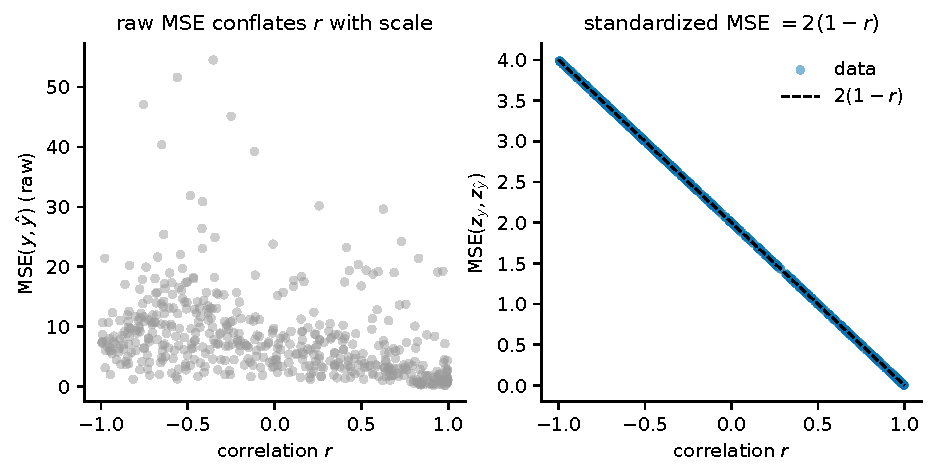
\includegraphics[width=\linewidth]{figures/fig1_geometry.pdf}}{}
\caption{Geometry of the standardized-MSE / Pearson identity (Proposition~\ref{prop:1}).}
\label{fig:geometry}
\end{figure}

\subsection{Affine calibration restores scale without changing rank}\label{sec:prop2}
Correlation is invariant to strictly increasing affine transformations of $\hat
y$: a model trained on $\mathcal{L}_{\mathrm{P}}$ controls the \emph{shape} of the
prediction but not its scale or offset. This is corrected exactly and cheaply.
\begin{proposition}\label{prop:2}
Let $p\in\mathbb{R}^n$ be raw predictions and $r=r(y,p)$. The affine map
$\tilde y = a\,p+b$ minimizing $\tfrac1n\sum_i (a p_i + b - y_i)^2$ has
\[
a^\star = \frac{\mathrm{cov}(y,p)}{\mathrm{var}(p)},\qquad
b^\star = \bar y - a^\star\,\bar p,\qquad
\mathrm{MSE}_{\min} = \sigma_y^2\,(1-r^2).
\]
If $a^\star>0$, the map is strictly increasing and hence preserves $r$, the
Spearman correlation, and every top-$k$/ranking quantity, while setting the
calibration slope to $1$ and intercept to $0$.
\end{proposition}
\begin{proof}
Ordinary least squares for a single predictor gives $a^\star,b^\star$ as stated;
the minimized residual variance of simple linear regression is
$\sigma_y^2(1-r^2)$. A strictly increasing transform preserves the order of $p$
and leaves correlation-type and rank-based statistics unchanged.
\end{proof}
We fit $(a^\star,b^\star)$ on held-out validation predictions (never on the test
set) and apply them to the test predictions. Isotonic regression provides a
monotone non-linear alternative when the raw-vs-true relationship is monotone but
curved. A positive affine map preserves $r$; a negative affine slope changes its
sign, and nonlinear isotonic calibration can change its magnitude. Calibration
can nonetheless improve RMSE, bias and slope (Figure~\ref{fig:simulation};
Section~\ref{sec:res-calibration}).

\begin{figure}[tbp]\centering
\IfFileExists{figures/fig2_simulation.pdf}{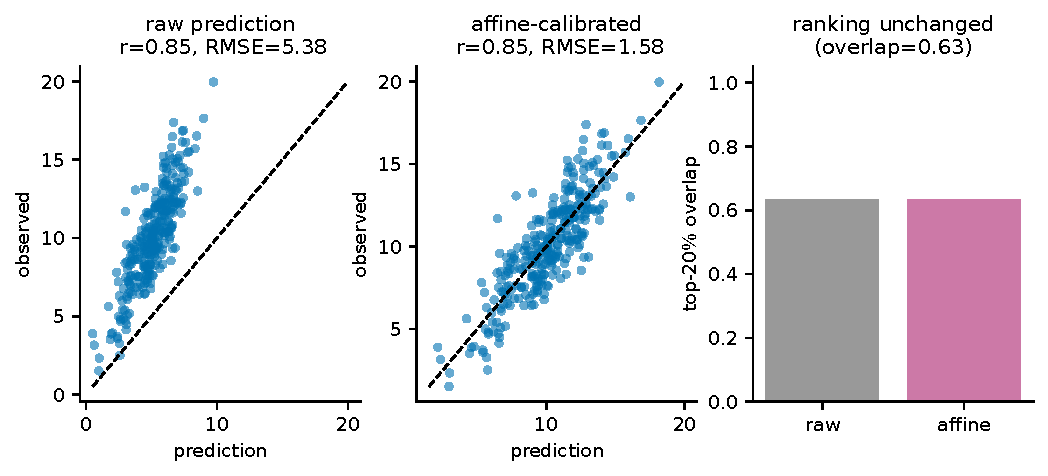
\includegraphics[width=\linewidth]{figures/fig2_simulation.pdf}}{}
\caption{Controlled simulation of Proposition~\ref{prop:2}: a well-correlated but
mis-scaled prediction (left) is corrected by affine calibration (middle) ---
RMSE falls while Pearson $r$ is unchanged --- and the top-$20\%$ selection
overlap is identical before and after (right).}
\label{fig:simulation}
\end{figure}

\subsection{Mini-batch versus global Pearson}\label{sec:prop3}
\begin{proposition}\label{prop:3}
For a partition of the data into batches $B_1,\dots,B_K$, the batch-averaged loss
$\tfrac1K\sum_k \bigl(1-r_{B_k}\bigr)$ is not equal to $1-r_{\mathrm{global}}$ in
general, because $r$ is a non-linear (ratio-of-moments) functional of the data.
Because the functional is nonlinear, neither equality nor a monotonic relation
between batch size and discrepancy is guaranteed without further assumptions.
\end{proposition}
A full-batch evaluation of $\mathcal{L}_{\mathrm{P}}$ optimizes the global
objective exactly; a large batch is an approximation, and smaller batches
optimize a noisier surrogate. A supporting experiment quantifies the practical
effect over the tested range.

\subsection{Multi-trait and group-aware variants}\label{sec:groupaware}
The loss extends naturally to $T$ traits, $\mathcal{L}=\tfrac1T\sum_{t=1}^T
(1-r_t)$ (or a weighted sum $\sum_t w_t(1-r_t)$), and to a group-aware objective
$\mathcal{L}=\tfrac1G\sum_{g=1}^G (1-r_g)$ where $g$ indexes environments, years,
families or sites --- aligning training with the within-environment correlation
that multi-environment breeding programs actually care about. As in
Proposition~\ref{prop:3}, neither variant equals the pooled global correlation.

\section{Materials and Methods}\label{sec:methods}

\paragraph{Datasets.} We use three public sources, for a total of \NUM{101}
trait--dataset combinations across \NUM{12} panels/sources spanning 10 species. (i) \emph{EasyGeSe}
\citep{quesada2025easygese}: a benchmark of ten species (barley, common bean,
lentil, maize, eastern oyster, pig, loblolly pine, rice, soybean and wheat)
providing genotypes, phenotypes and \emph{fixed} cross-validation partitions; the
maize set is the global genotype-by-environment competition panel
\citep{washburn2025maize}. (ii) The CIMMYT \emph{wheat} panel
\citep{crossa2010}: 599 lines, 1{,}279 DArT markers and grain yield in four
environments, analyzed as four outcomes. (iii) \emph{SoyNAM}
\citep{xavier2016soynam}: $\sim$5{,}500 recombinant inbred lines in 40 biparental
families, analyzed for four agronomic traits. Genotypes are coded as allele
dosages; preprocessing (unsupervised, no phenotype) applies a minor-allele
frequency filter ($\geq 0.01$), mean imputation, and a top-variance cap at
20{,}000 markers for the seven panels whose marker count exceeded 20{,}000
(barley, lentil, maize, oyster, pig, rice and soybean).
Table~\ref{tab:datasets} and Figure~\ref{fig:datasets} summarize the data.

\begin{table}[t]\centering
\caption{The 101 trait--dataset combinations across 12 panels/sources (10 species;
10 panels from EasyGeSe, plus CIMMYT wheat and SoyNAM). $n$ is the number of genotypes, $p$ the markers used
(after MAF filtering and the 20{,}000-marker variance cap), and GBLUP $r$ the mean
within-dataset predictive ability of GBLUP (a difficulty index).}\label{tab:datasets}
\begin{tabular}{lrrrrl}
\toprule
Species & $n$ & $p$ & traits & GBLUP $r$ & source\\
\midrule
rice & 352 & 20{,}000 & 36 & 0.46 & EasyGeSe \\
pine & 925 & 4{,}421 & 17 & 0.82 & EasyGeSe \\
wheatG & 371 & 12{,}546 & 16 & 0.59 & EasyGeSe \\
maize & 4421 & 20{,}000 & 6 & 0.83 & EasyGeSe \\
bean & 444 & 16{,}707 & 5 & 0.57 & EasyGeSe \\
lentil & 324 & 20{,}000 & 5 & 0.79 & EasyGeSe \\
soybeanNAM & 5487 & 4{,}401 & 4 & 0.71 & SoyNAM \\
wheat & 599 & 1{,}279 & 4 & 0.46 & BGLR/CIMMYT \\
barley & 1438 & 20{,}000 & 2 & 0.58 & EasyGeSe \\
oyster & 372 & 20{,}000 & 2 & 0.38 & EasyGeSe \\
pig & 1709 & 20{,}000 & 2 & 0.31 & EasyGeSe \\
soybean & 346 & 20{,}000 & 2 & 0.40 & EasyGeSe \\
\bottomrule
\end{tabular}

\vspace{2pt}
{\footnotesize\raggedright The count of 12 panels/sources (spanning 10 species)
treats related germplasm
sharing a common crop as distinct panels: wheatG (EasyGeSe) and wheat (CIMMYT) are
separate sources, as are soybean (EasyGeSe) and soybeanNAM (SoyNAM)
panels of the same species drawn from different sources.\par}
\end{table}

\begin{figure}[tbp]\centering
\IfFileExists{figures/fig3_datasets.pdf}{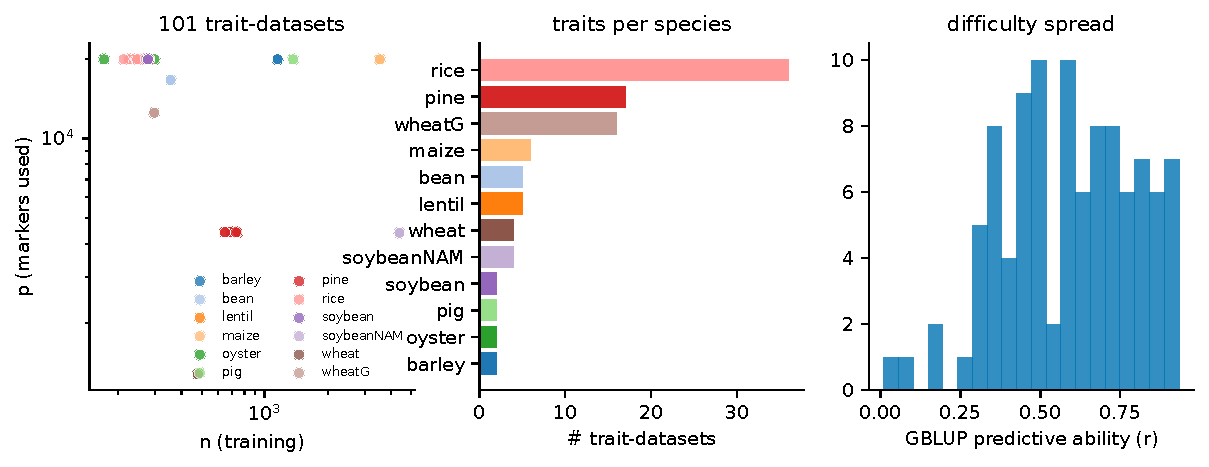
\includegraphics[width=\linewidth]{figures/fig3_datasets.pdf}}{}
\caption{Dataset map: size, dimensionality and predictability across species.}
\label{fig:datasets}
\end{figure}

\paragraph{Models.} The parametric baseline is GBLUP with REML-estimated variance
components, implemented in the spectral basis of the linear genomic kernel
$K=XX^\top/p$ and validated against the \texttt{rrBLUP} package
\citep{endelman2011} to floating-point precision (cross-implementation
correlation $1.0000$). We also include ridge regression as a linear baseline. The neural predictors
are a multilayer perceptron (MLP), a one-dimensional convolutional network over
ordered markers (1D-CNN), a light Transformer over marker patches, and four
protocol-matched, literature-inspired adaptations: DeepGS
\citep{ma2018deepgs}, DNNGP \citep{wang2023dnngp}, PNNGS \citep{pnngs2024}, and
SoyDNGP \citep{gao2023soydngp}. These are not exact reproductions: they retain
published motifs while using common dosage inputs, preprocessing, training and
evaluation. For the primary ablation, one configuration is selected per dataset
registry key and architecture under MSE and frozen across losses. EasyGeSe and
CIMMYT use one representative trait per panel and transfer it to the other
traits; the four SoyNAM phenotypes are separate registry keys and are tuned on
their own phenotype. The contrast changes only the loss conditional on the
configuration, but selection under MSE may favor MSE.

\paragraph{Loss functions.} We compare MSE; the standardized-MSE Pearson loss
$1-r$ (Proposition~\ref{prop:1}); a hybrid $\,(1-r)+\lambda\,\mathrm{MSE}\,$ with
$\lambda=0.1$; and a concordance-correlation loss $1-\rho_c$ \citep{lin1989},
which penalizes correlation, scale and offset jointly. The negative-Pearson and
explicit standardized-MSE forms are included in the numerical checks.

\paragraph{Calibration.} For every model and loss we report predictions under
three post-hoc maps: raw (identity), affine (Proposition~\ref{prop:2}) and
isotonic. Calibrators are fit on validation predictions only.

\paragraph{Cross-validation.} We use the fixed EasyGeSe partitions (5 folds
$\times$ 2 repeats $=$ 10 folds per trait) and repeated $K$-fold for wheat and
SoyNAM. Within each training fold an inner 80/20 split provides early-stopping and
calibration data; markers are standardized with training statistics only;
targets are standardized with training statistics for the neural networks and
predictions are returned in the original units. Neural networks early-stop on the
validation value of the loss being trained. The test fold is never used for
fitting, early stopping or calibration. Primary hyper-parameters, however, were
selected before outer CV on the full tuning phenotype described above, so
absolute performance is not a nested estimate. In a separate CIMMYT sensitivity,
MSE and Pearson each received the same eight-candidate bank inside five outer
folds using only environment-1 outer-training observations; configurations were
evaluated in four environments with three initialization seeds.

\paragraph{Evaluation metrics.} Predictive: Pearson $r$, Spearman $\rho$, RMSE,
MAE, $R^2$, mean bias, and the calibration slope and intercept (ideal $1$ and
$0$). Upper-tail ranking, at intensities $k\in\{5,10,15,20\}\%$: top-$k$ overlap,
precision@$k$, recall@$k$, NDCG@$k$ \citep{jarvelin2002ndcg}, selection
differential, mean phenotype of the selected, and relative efficiency (achieved
upper-tail differential divided by the oracle differential). Larger phenotypes
are always the target; these metrics are not interpreted as breeding gain when
lower or intermediate values are desirable.

\paragraph{Statistical analysis.} For each task, architecture and loss we first
average the ten fold values and form
$\Delta m=m_{\mathrm{loss}}-m_{\mathrm{MSE}}$. The pooled contrast averages the
seven architectures within task. The primary estimand gives equal weight to each
of 12 panels; a trait-weighted estimand is a sensitivity check. Confidence
intervals resample panels as clusters (20,000 replicates), and an exact two-sided
sign-flip test reverses all task contrasts within a panel together.
Leave-one-panel-out ranges assess influence. A corroborative mixed model of the
paired deltas contains loss, architecture, their interaction, panel as a blocking
factor and a random task intercept; a likelihood-ratio test compares models with
and without the interaction. Raw Pearson is the prespecified primary endpoint,
raw NDCG@$10$ is secondary, and RMSE is normalized by the test-fold phenotype
standard deviation after validation-fitted affine calibration. The nested-HPO
experiment covers MLP, CNN and Transformer only and is analyzed separately and descriptively because its environments,
folds and seeds are repeated measures from one wheat panel.

\paragraph{Implementation.} The framework is released as the Python package
\texttt{ccgp}, built on PyTorch \citep{paszke2019pytorch}, scikit-learn
\citep{pedregosa2011sklearn} and NumPy
\citep{harris2020numpy}, with the neural networks trained using the Adam optimizer
\citep{kingma2015adam}, deterministic split definitions and recorded tuned
configurations. The main campaign used one initialization per fold; only the
nested wheat sensitivity used three seeds. Analysis scripts validate the
90,900-row campaign and 1,080-row nested result files before producing tables
and machine-readable figure source data.

\section{Results}\label{sec:results}

\subsection{Numerical validation}\label{sec:res-numerical}
Across 80 simulated cases, the implemented Pearson loss, $1-r$, and one half of
the standardized MSE agreed to a maximum absolute difference of
$5.0\times10^{-8}$ (mean $7.4\times10^{-9}$). The affine residual identity in
Proposition~\ref{prop:2} agreed to $1.2\times10^{-15}$ over 200 cases. Both the
Pearson and concordance losses passed automatic gradient checks, and $-r$ and
$1-r$ had identical gradients. These checks establish numerical equivalence,
not empirical superiority.

\subsection{Headline result: correlation, calibration and selection separate}\label{sec:res-loss}

\ifdefined\GTHREE\else
\begin{figure}[tbp]\centering
\IfFileExists{figures/fig4_loss_comparison.pdf}{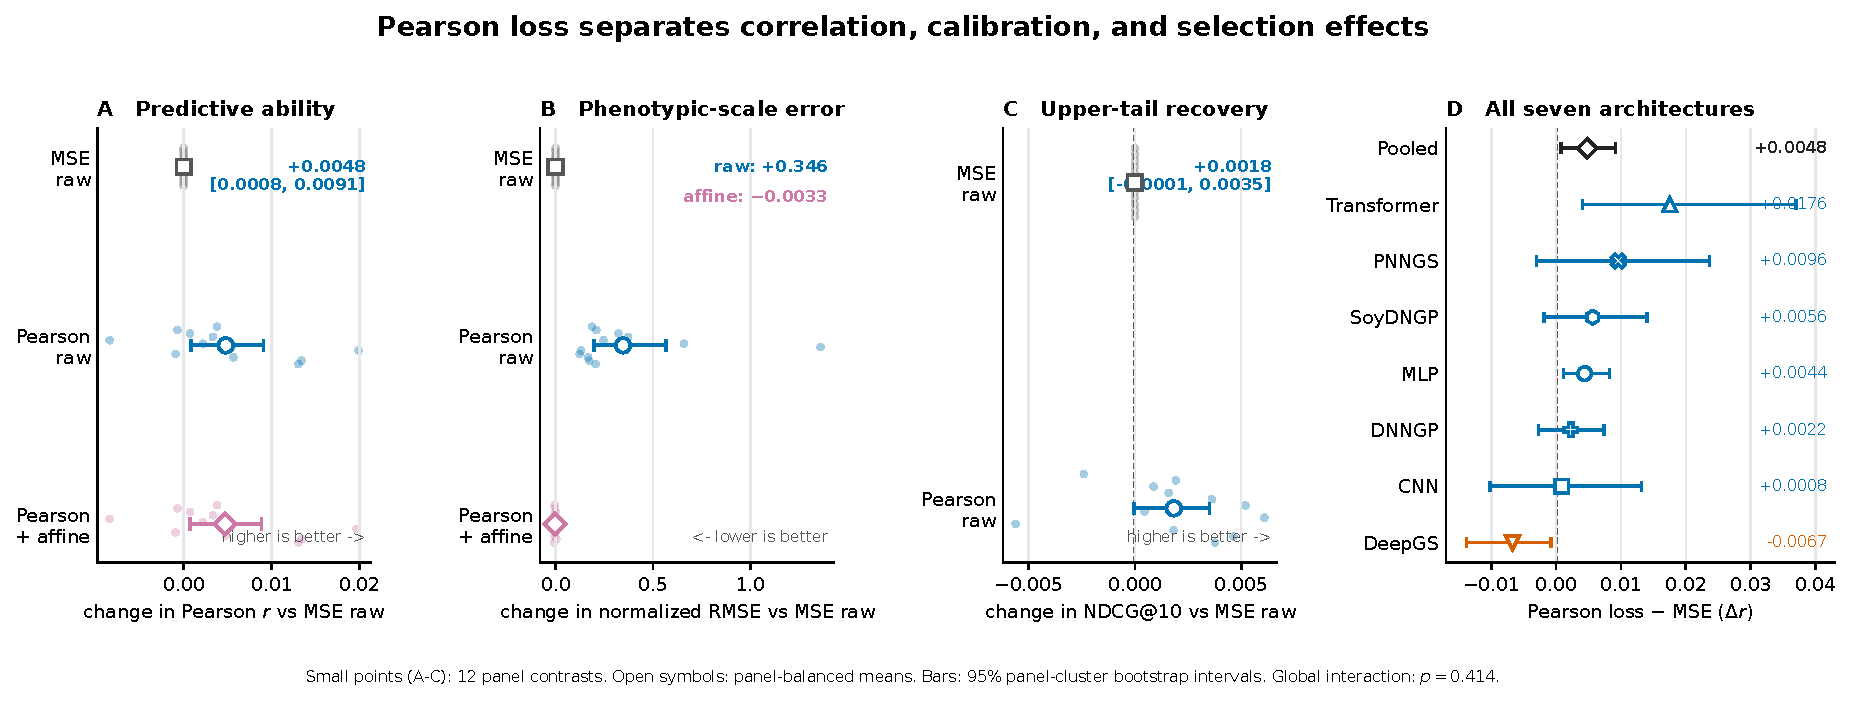
\includegraphics[width=\linewidth]{figures/fig4_loss_comparison.pdf}}{}
\caption{The paper's central comparison. Panels A--B compare the scale-aware
raw MSE baseline, the correlation-targeted but unscaled raw Pearson output, and
the validation-fitted affine Pearson output; Panel C compares raw MSE and raw
Pearson predictions for upper-tail recovery. Small points are contrasts for
each of 12 panels, open symbols are panel-balanced means, and bars are 95\%
panel-cluster bootstrap intervals. Raw Pearson predictions gain $0.0048$ in $r$
but lose $0.346$ in normalized RMSE; affine calibration retains a $0.0047$
correlation gain and changes normalized RMSE by $-0.0033$. The raw NDCG@$10$
change is only $+0.0018$. Panel D reports the Pearson-minus-MSE correlation
contrast, interval and exact point estimate for
the pooled result and every neural architecture in the main benchmark. Folds
were averaged within 101 tasks and architectures within task before panels were
weighted equally.}
\label{fig:loss}
\end{figure}
\fi

Figure~\ref{fig:loss} summarizes the practical sequence. Relative to the
MSE-trained raw baseline, Pearson-trained raw predictions gained $0.0048$ in
correlation but increased normalized RMSE by $0.346$ (95\% panel-cluster
bootstrap interval $[0.1965,0.5675]$), because correlation training does not
identify scale or offset. Validation-fitted affine calibration retained nearly
all of the correlation gain ($+0.0047$) and brought normalized RMSE back to the
MSE baseline ($-0.0033$, $[-0.0062,0.0000]$). Thus the headline is not that
Pearson replaces MSE on every criterion: it slightly improves the target
correlation, a separate calibration step is needed for phenotypic-scale
predictions, and the decision-level effect must be checked directly.

The final grid contained 90,900 rows: seven neural architectures, four losses,
101 tasks, ten test folds and three calibration maps, plus GBLUP and ridge
baselines. All architectures covered the same 101 tasks. After folds were
averaged, the panel-balanced Pearson-minus-MSE contrast for raw test correlation
was $\Delta r=+0.0048$ (95\% panel-cluster bootstrap interval
$[0.0008,0.0091]$). Seventy-eight of 101 task-level pooled
contrasts were positive. An exact test that flipped the signs of all tasks
within each panel gave $p=0.052$, appropriately reflecting that only 12 panels,
not 707 independent experiments, were observed. Weighting every trait equally
instead produced $+0.0101$ ($[0.0028,0.0158]$), showing that the estimate is
sensitive to the many traits contributed by rice, pine and wheatG.

The hybrid and CCC losses gave panel-balanced $\Delta r$ values of $+0.0055$
($[0.0010,0.0100]$) and $+0.0078$ ($[0.0022,0.0139]$), respectively. Figure~\ref{fig:loss}D
reports all seven architecture-specific Pearson contrasts and intervals. The
Transformer has the largest positive estimate ($+0.0176$), while DeepGS is a
negative counterexample ($-0.0067$); PNNGS and SoyDNGP are positive but
uncertain, MLP shows a smaller positive estimate, and DNNGP and CNN lie near
zero. The apparent spread is descriptive: the global loss-by-architecture test
is inconclusive ($\chi^2_{12}=12.40$, $p=0.414$). The four named networks are
literature-inspired adaptations, not exact reproductions of the published systems.

\subsection{Ranking and scale}\label{sec:res-selection}
Pearson training changed panel-balanced raw NDCG@$10$ by only $+0.0018$
($[-0.0001,0.0035]$) and upper-tail overlap by $+0.0033$
($[-0.0010,0.0069]$). CCC gave the largest, still small, NDCG contrast
($+0.0034$, $[0.0015,0.0056]$). These quantities recover the highest observed
phenotypes; because trait desirability was not harmonized, they must not be read
as realized breeding gain for traits where lower values are preferred. Ridge
and GBLUP retained the best mean ranks for both Pearson and NDCG@$10$. The weak
ranking response is therefore an empirical result in its own right: a measurable
gain in global predictive ability did not substantially change which candidates
would be recovered by the upper-tail rule used here.

Affine-calibrated NRMSE, defined as RMSE divided by the test-fold phenotype
standard deviation, was essentially unchanged by Pearson training
($-0.0011$, $[-0.0036,0.0015]$) or the hybrid loss ($-0.0018$,
$[-0.0041,0.0006]$). CCC produced $-0.0028$ ($[-0.0054,-0.0003]$), a very small
normalized-error reduction. Absolute RMSE values were not pooled across traits
because their measurement units differ.

\subsection{Calibration}\label{sec:res-calibration}

\ifdefined\GTHREE\else
\begin{figure}[tbp]\centering
\IfFileExists{figures/fig5_calibration.pdf}{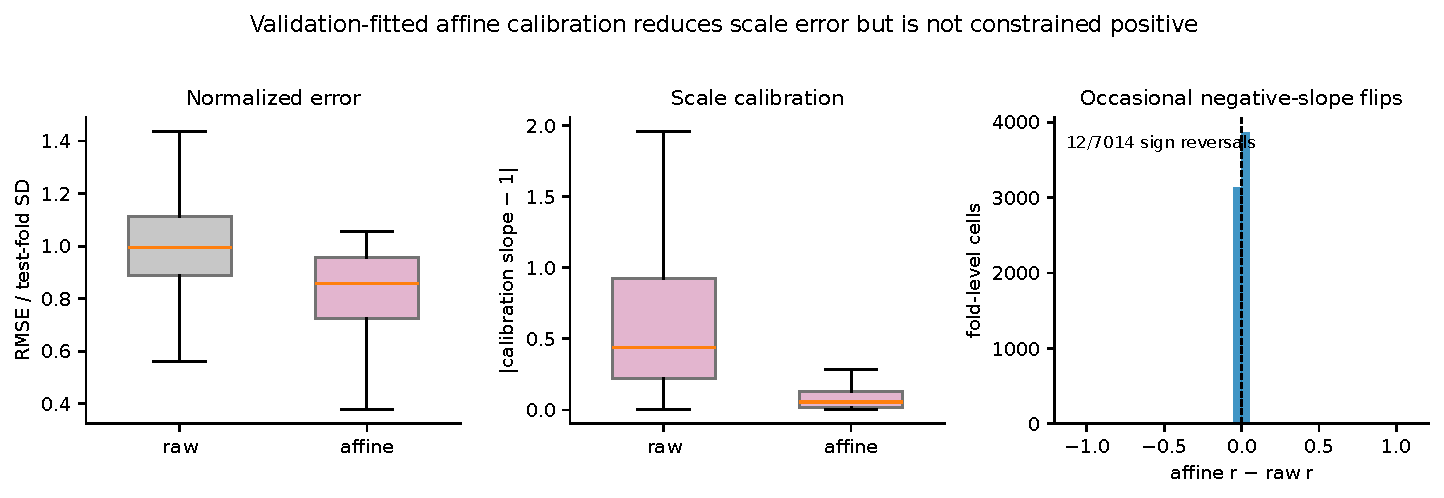
\includegraphics[width=\linewidth]{figures/fig5_calibration.pdf}}{}
\caption{Validation-fitted affine calibration for Pearson-trained networks.
Boxplots summarize 707 task--architecture means (outliers omitted visually);
the histogram uses 7,014 fold-level cells with finite raw and affine
correlations. Calibration reduced normalized error and slope deviation, but 12
folds (0.17\%) had a validation-fitted negative slope that reversed the sign of
test-set correlation.}
\label{fig:calibration}
\end{figure}
\fi

Across Pearson-trained networks, mean RMSE fell from 10.54 to 7.99 after affine
calibration and the median calibration slope moved from 0.918 to 0.957. These
raw-unit averages are descriptive only. A positive affine map preserves ranks,
but the implementation used the unconstrained least-squares slope estimated on
validation data. Among 7,014 comparable fold cells, 12 (0.17\%) therefore
reversed the sign of test correlation. Loss comparisons for correlation and upper-tail recovery use raw predictions.
Figure~\ref{fig:loss} additionally audits raw versus affine correlation to check
that calibration retains the gain. Scale outcomes use affine predictions.

\subsection{Loss-specific HPO and seed sensitivity}\label{sec:res-nested}

\ifdefined\GTHREE\else
\begin{figure}[tbp]\centering
\IfFileExists{figures/fig6_meta.pdf}{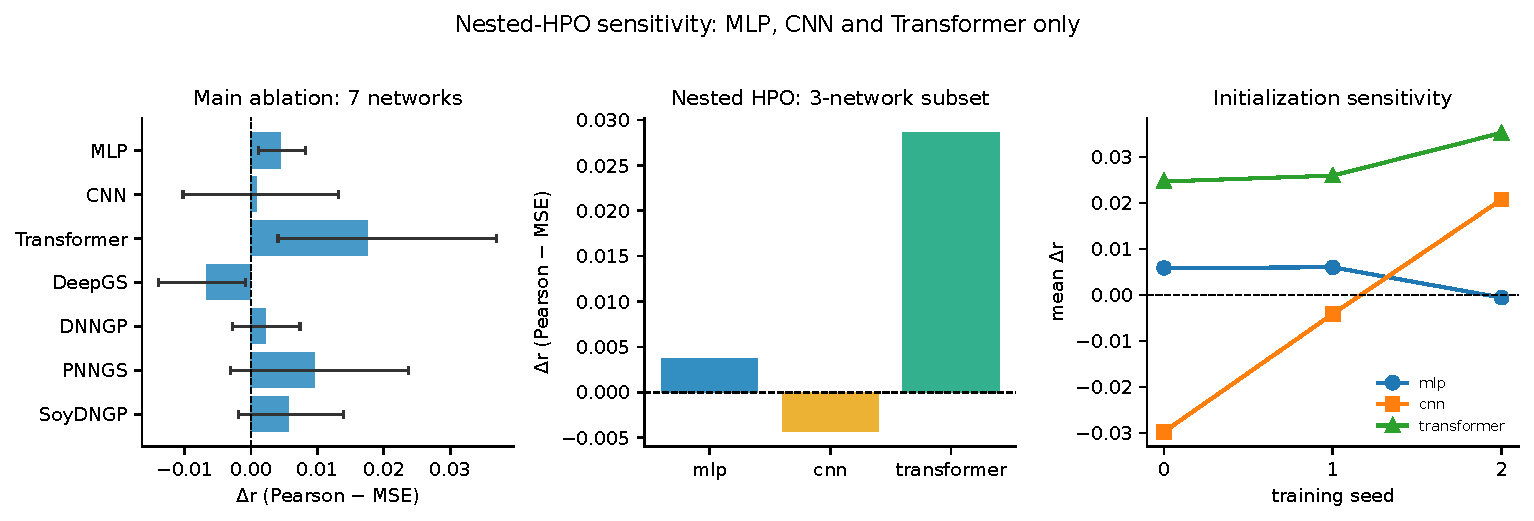
\includegraphics[width=\linewidth]{figures/fig6_meta.pdf}}{}
\caption{Sensitivity to tuning and initialization. The shared-HPO panel shows
panel-balanced effects for all seven networks in the 101-task benchmark. The
nested-HPO and seed panels contain only MLP, CNN and Transformer because
loss-specific nested tuning was run only for these three generic architectures;
the four literature-inspired networks were not evaluated in this sensitivity.
Nested means cover four CIMMYT wheat environments, five outer folds and three
seeds; configurations were selected separately for MSE and Pearson using only
environment-1 observations in each outer-training set. The repeated wheat
outcomes are not independent replications and no confirmatory $p$-value is assigned.}
\label{fig:meta}
\end{figure}
\fi

The nested sensitivity contained 1,080 prediction rows. It was run only for
MLP, CNN and Transformer; DeepGS, DNNGP, PNNGS and SoyDNGP therefore have no
loss-specific nested-HPO result, rather than an omitted result (Figure~\ref{fig:meta}).
Across the three tested architectures, loss-specific Pearson tuning changed raw $r$ by $+0.0093$ on
average. Estimates were $+0.0286$ for the Transformer, $+0.0038$ for the MLP,
and $-0.0044$ for the CNN. Corresponding NDCG@$10$ contrasts were $+0.0069$,
$+0.0071$, and $-0.0060$. CNN's mean $\Delta r$ moved from $-0.0297$ to
$-0.0041$ to $+0.0207$ across seeds 0--2; Transformer remained positive
($+0.0246$, $+0.0259$, $+0.0352$). Thus objective-specific tuning supports the
Transformer signal but also demonstrates initialization uncertainty that the
single-seed main campaign cannot quantify.


\section{Discussion}\label{sec:discussion}

\subsection{A valid objective with a modest empirical effect}
The algebraic result is exact: minimizing standardized MSE maximizes Pearson
correlation. The empirical result is more restrained. Once all seven networks
are evaluated on the same 101 tasks and panels are equally weighted, Pearson
training improves $r$ by about five thousandths. The cluster-bootstrap interval
is positive, but an exact 12-panel sign-flip test lies at the conventional
threshold. The raw Pearson outputs pay a large scale penalty; validation-fitted
affine calibration removes it while leaving the correlation gain essentially
intact. NDCG changes are smaller still. This sequence---align the objective,
then restore scale---and the distinction between mathematical alignment and
modest practical gain are the paper's main findings.

Trait weighting matters. A trait-weighted analysis gives twice the
panel-balanced effect because rice, pine and wheatG contribute many phenotypes.
Neither estimand is intrinsically wrong: the first describes an average listed
trait and the second an average panel. We use panel balance for the headline to
avoid allowing heavily phenotyped resources to determine a cross-panel claim,
and report both for transparency.

\subsection{Architecture heterogeneity is suggestive, not universal}
The Transformer repeatedly shows the largest positive estimate, including after
loss-specific nested tuning. MLP gains are small, CNN is near zero after panel
balance, and the DeepGS-inspired network becomes worse under Pearson training.
This counterexample rules out a universal optimization advantage. At the same
time, the omnibus loss-by-architecture interaction is not significant, so the
apparent ordering should be treated as hypothesis-generating rather than as a
formal taxonomy of networks. Possible mechanisms include different curvature,
normalization and early-stopping behavior, but the present benchmark does not
identify them.

The four named systems are protocol-matched, literature-inspired adaptations.
DeepGS retains a marker convolution/dense motif but adds batch normalization;
DNNGP is genotype-only and uses PCA rather than reproducing its complete
multi-omic setting; PNNGS retains parallel residual kernels but changes the
stem, pooling and validation protocol; and SoyDNGP converts dosage vectors to a
96$\times$96 one-channel representation rather than the published
206$\times$206$\times$3 encoding. Their results evaluate whether these motifs
respond to the loss under one common protocol, not whether the original papers
would reproduce identically.

\subsection{Correlation, calibration and upper-tail recovery}
Correlation is invariant to positive affine transformations, making scale
calibration a separate problem. Validation-fitted affine calibration reduced
normalized error in aggregate, but unconstrained least squares occasionally
estimated a negative slope and reversed rankings. A production implementation
should constrain the slope to be positive or fall back to an intercept-only
map. We avoided this ambiguity by using raw outputs for correlation and ranking
and affine outputs only for scale outcomes.

The upper-tail metrics answer a narrower question than biological selection.
They quantify recovery of the largest observed phenotypes. Some disease,
maturity and moisture traits favor lower or intermediate values, and the public
metadata did not provide a uniform desirability direction. Consequently these
metrics cannot establish breeding utility without trait-specific economic
weights and target directions. Their weak improvement nevertheless shows that a
small gain in global correlation need not translate into a substantial change
in the selected set, consistent with earlier ranking-based critiques
\citep{ornella2014,blondel2015}.

\subsection{What the HPO comparison does and does not show}
The main experiment is a controlled shared-configuration ablation. For each
panel and architecture, a configuration selected under MSE on one representative
trait was transferred to all traits and frozen across losses. This isolates the
training objective conditional on that configuration, but it can favor MSE and
uses the tuning phenotype before outer evaluation; it is not nested
performance estimation. The separate CIMMYT experiment selects MSE and Pearson
configurations inside each outer-training set from identical candidate banks.
Its Transformer result is directionally consistent with the main analysis, but
the experiment tunes on environment 1, transfers to four correlated wheat
environments, and covers only three architectures. It is a sensitivity analysis,
not a second general benchmark.

\subsection{Limitations and future work}
The main campaign uses one neural initialization per fold. The three-seed wheat
analysis shows that this is a material limitation, especially for CNN. Future
work should repeat all task--architecture cells over seeds, nest tuning within
every outer fold and phenotype, and record the full HPO trial ledger rather than
only selected configurations. With only 12 panels, resampling uncertainty also
remains coarse even though folds and architectures are not treated as independent
replicates.

The marker filter, imputation and variance cap were fitted transductively on the
full genotype matrix but without phenotypes; fold-specific standardization was
then fitted on training individuals. Binary, ordinal and continuous phenotypes
were analyzed together for breadth, although Gaussian calibration and RMSE have
different meanings across these scales. Constant or nearly constant test folds
also generated missing correlations, concentrated in rice seed color. These
limitations motivate stratified future benchmarks.

Finally, the benchmark compares objective functions, not every possible neural
architecture, and linear baselines remain strongest by mean rank. The practical
recommendation is therefore conservative: try Pearson or CCC as a paired
objective ablation when correlation is the operational endpoint; retain MSE and
linear baselines; calibrate separately when phenotypic scale matters; and verify
the actual trait-specific selection decision rather than inferring it from $r$.


\section{Conclusion}
A standardized-MSE Pearson loss aligns neural-network training with the
predictive-ability metric used throughout genomic prediction; because correlation
is scale-free, a separate calibration step or a scale-aware objective is needed
when calibrated phenotypic values matter; and global correlation should be
complemented by decision-specific metrics. Empirically, across 101 trait--datasets the average
benefit is small, sensitive to panel weighting, and not uniform across
architectures. The clearest descriptive signal occurs for the Transformer,
while DeepGS provides a negative counterexample, and no neural loss unseated
GBLUP or ridge on mean rank. Together, these results provide a practical
framework for separating objective alignment, phenotypic calibration and
decision-level evaluation in neural genomic prediction; Pearson or CCC should be
viewed as objective-specific alternatives to test alongside MSE rather than as
universal replacements.

\section*{Data availability}
All datasets are public: EasyGeSe (Zenodo, DOI \texttt{10.5281/zenodo.15348871}), the CIMMYT wheat panel
(\texttt{BGLR} R package \citep{perez2014bglr}) and SoyNAM (\texttt{SoyNAM} R package). Code, fixed
cross-validation partitions, tuned configurations and a recorded runtime manifest are
released as the \texttt{ccgp} package, with source at
\url{https://github.com/GBeurier/gs-loss} (a versioned archive will be
deposited at Zenodo, DOI to be assigned). All datasets used in the reported
benchmark are public and download automatically. Supporting Information (File~S1,
\texttt{supplement.pdf}) documents the architecture adaptations, complete paired
contrasts, missingness, HPO provenance, calibration, mean ranks and nested wheat
sensitivity. Machine-readable source tables accompany every data-driven figure.

\bibliographystyle{apalike}
\bibliography{refs}



\end{document}
"  for a
% line-numbered bioRxiv preprint; default (0) is the clean submission build.
\providecommand{\PREPRINTMODE}{0}
\ifnum\PREPRINTMODE=1 \usepackage[switch]{lineno}\fi

\theoremstyle{plain}
\newtheorem{proposition}{Proposition}
\theoremstyle{remark}
\newtheorem{remark}{Remark}

\title{\bfseries Metric-consistent neural networks for genomic prediction and
selection: a standardized-MSE Pearson loss, affine calibration, and
selection-aware evaluation}

\author[1,2]{Gr\'egory Beurier\thanks{Corresponding author: \texttt{gregory.beurier@cirad.fr}}}
\author[1,2]{Denis Cornet}
\author[1,2]{Lauriane Rouan}
\author[1,2]{David Cros}
\affil[1]{CIRAD, UMR AGAP Institut, Montpellier, France}
\affil[2]{UMR AGAP Institut, Univ Montpellier, CIRAD, INRAE, Institut Agro, Montpellier, France}
\date{\ifnum\PREPRINTMODE=1 \textit{Preprint --- not peer-reviewed} \quad\textbullet\quad \today\else\today\fi}

\begin{document}
\maketitle
\ifnum\PREPRINTMODE=1 \linenumbers \fi

\begin{abstract}
\noindent
Genomic prediction involves three objectives that are often conflated:
association with phenotype, calibration to the phenotypic scale, and recovery of
selection candidates. Neural predictors are usually trained by mean squared
error (MSE), although predictive ability is commonly evaluated by Pearson
correlation and candidate ranking. We use the identity
$\mathrm{MSE}(z_y,z_{\hat y})=2(1-r)$ to implement a stable differentiable
Pearson objective and ask what is gained, and what is not, by aligning the
training objective with the correlation metric. A shared-configuration ablation compared MSE,
Pearson, hybrid and concordance-correlation losses for seven architectures on
101 public trait--dataset tasks from 12 panels spanning ten species. Folds were
averaged before inference; effects were balanced across panels and uncertainty
was obtained by panel-cluster bootstrap. Relative to MSE, Pearson training gave
a small positive raw-correlation estimate of $0.0048$ (95\% cluster bootstrap
interval $0.0008$--$0.0091$), while an exact 12-panel sign-flip test was just
above the conventional threshold ($p=0.052$). Raw Pearson predictions were
poorly scaled (normalized-RMSE change $+0.346$ relative to raw MSE), but
validation-fitted affine calibration removed this penalty ($-0.0033$) without
materially changing correlation. The corresponding change in NDCG@$10$ was
only $0.0018$ ($-0.0001$--$0.0035$). Estimates varied across architectures: the Transformer had
the clearest positive contrast ($+0.0176$), whereas the DeepGS-inspired network
had a negative contrast ($-0.0067$); the global loss-by-architecture interaction
was inconclusive. A separate loss-specific nested-HPO sensitivity for MLP, CNN
and Transformer on CIMMYT wheat supported a Transformer signal but not a uniform benefit and revealed
material seed variability. Affine calibration restored phenotypic scale, although an
unconstrained negative validation slope occasionally reversed rankings. Thus a
differentiable Pearson loss is feasible, but metric-consistent training is most
useful as part of a workflow in which objective alignment, calibration and
selection performance are evaluated separately rather than as a universal
replacement for MSE.

\end{abstract}

\section{Introduction}

Genomic selection \citep{meuwissen2001} predicts the genetic merit of candidate
individuals from genome-wide markers, and has become central to modern plant and
animal breeding \citep{heffner2009,jannink2010,desta2014}. The dominant
parametric baseline, genomic best linear unbiased prediction
(GBLUP)/ridge-regression BLUP \citep{vanraden2008,endelman2011}, is increasingly
complemented by machine-learning and deep-learning predictors
\citep{ma2018deepgs,wang2023dnngp,montesinos2021review,montesinos2021power}.
Whether deep learning improves on GBLUP remains dataset-dependent: recent
comparisons find that neither systematically dominates, and that outcomes hinge
on tuning, architecture and the choice of evaluation metric
\citep{montesinos2025dlgblup}.

That last point is the subject of this paper. Genomic predictors are trained, by
near-universal default, to minimize the mean squared error (MSE). But they are
\emph{assessed} with the Pearson correlation $r$ between predicted and observed
phenotypes --- the ``predictive ability'' reported in essentially every genomic
prediction study \citep{crossa2010} --- and they are \emph{used} to rank
candidates and select the best ones. There is therefore a systematic mismatch
between the training objective and one of the principal metrics used to evaluate
genomic prediction. More importantly, neither MSE nor Pearson correlation is
identical to the ranking problem ultimately faced in selection.
\citet{waldmann2019} showed that selecting a model by $r$ can disagree with
selecting it by MSE or $R^2$. \citet{ornella2014} argued that $r$ is a poor guide
to performance in the tails of the distribution, where selection actually
operates, and evaluated the recovery of the best $\alpha\in\{10,\dots,40\}\%$ of
individuals. \citet{blondel2015} reframed genomic selection as a ranking problem,
introduced NDCG from information retrieval as an accuracy measure, and reported
that $r$ correlates poorly with ranking quality.

If correlation is the target, why not train for it directly? A recent
convolutional architecture for genomic selection states plainly that ``Pearson
correlation cannot be set as the loss function'' and substitutes a family of
$L_p$ losses \citep{pnngs2024}. We show this premise is false. The Pearson
correlation \emph{is} a loss --- a standardized MSE --- and training with it is
both well posed and numerically stable. The remaining objection to a correlation
loss, that it ignores scale and offset, is real but easily and provably remedied
by an affine recalibration applied after training.

The empirical question therefore has a simple three-stage structure: compare
the usual MSE-trained raw predictions with Pearson-trained raw predictions to
measure correlation alignment, then calibrate the Pearson outputs on validation
data to recover phenotypic scale, and finally evaluate separately whether
correlation-aligned training changes upper-tail selection. Figure~\ref{fig:loss}
carries this structure through to the headline result.

\paragraph{Contributions.}
\begin{enumerate}
\item \textbf{A standardized-MSE Pearson loss (Section~\ref{sec:prop1}).} We give
the exact identity $\mathrm{MSE}(z_y,z_{\hat y}) = 2(1-r)$ and use it as a stable,
differentiable training objective, verified numerically (to single-precision
tolerance for the loss; to float64 machine precision for the calibration identity).
\item \textbf{Affine calibration with a closed form
(Section~\ref{sec:prop2}).} We prove that the optimal post-hoc affine map yields
residual error $\sigma_y^2(1-r^2)$ on the fitting sample and restores scale and
offset while preserving $r$ and rankings whenever the fitted slope is positive.
\item \textbf{Mini-batch analysis (Section~\ref{sec:prop3}).} We show the
mini-batch Pearson loss is a biased surrogate for the global objective and
quantify the effect of batch size empirically.
\item \textbf{A reproducible, selection-aware benchmark
(Sections~\ref{sec:methods}--\ref{sec:results}).} Across \NUM{101}
trait--datasets from \NUM{12} panels/sources spanning 10 species, with architecture, splits and tuning held
fixed so that only the loss changes, we report both predictive and
selection-oriented metrics, a confirmatory mixed-model analysis, and a
meta-analysis of \emph{when} correlation-consistent training helps. All data are
public and all code, splits and tuned configurations are released.
\end{enumerate}

\noindent We do not claim that a Pearson loss is uniformly superior to MSE; that
would be false. We provide a principled, reproducible framework for training,
calibrating and evaluating neural genomic predictors by treating predictive correlation,
phenotypic scale and selection as related but distinct objectives.

\section{Theory}\label{sec:theory}
Throughout, $y,\hat y\in\mathbb{R}^n$, with sample means $\bar y,\bar{\hat y}$ and
population variances $\sigma_x^2 = \tfrac1n\sum_i (x_i-\bar x)^2$. The Pearson
correlation is $r=r(y,\hat y)=\tfrac1n\sum_i z_{y,i} z_{\hat y,i}$ where
$z_{x,i}=(x_i-\bar x)/\sigma_x$ is the standardized variable.

\subsection{The Pearson loss is a standardized MSE}\label{sec:prop1}
\begin{proposition}\label{prop:1}
For non-degenerate $y,\hat y$ (i.e.\ $\sigma_y,\sigma_{\hat y}>0$),
\[
\mathrm{MSE}(z_y,z_{\hat y}) \;=\; \tfrac1n\sum_{i=1}^n (z_{y,i}-z_{\hat y,i})^2
\;=\; 2\,(1-r).
\]
Consequently $1-r = \tfrac12\,\mathrm{MSE}(z_y,z_{\hat y})$, and minimizing the
standardized MSE is exactly maximizing the Pearson correlation.
\end{proposition}
\begin{proof}
Expanding the square,
$\tfrac1n\sum_i (z_{y,i}-z_{\hat y,i})^2
= \tfrac1n\sum_i z_{y,i}^2 - 2\tfrac1n\sum_i z_{y,i} z_{\hat y,i}
+ \tfrac1n\sum_i z_{\hat y,i}^2 = 1 - 2r + 1 = 2(1-r)$,
because $\tfrac1n\sum_i z_{x,i}^2 = 1$ by construction and
$\tfrac1n\sum_i z_{y,i} z_{\hat y,i}=r$.
\end{proof}
This gives the loss $\mathcal{L}_{\mathrm{P}}(\hat y,y) = 1-r(\hat y,y)$,
implemented directly with a small $\varepsilon$ guarding the standard-deviation
denominators and numerically equivalent to
$\tfrac12\,\mathrm{MSE}(z_y,z_{\hat y})$. It is differentiable everywhere
$\sigma_{\hat y}>0$; we verify the gradient against finite differences and verify
the identity to single-precision tolerance in Section~\ref{sec:res-numerical}. The
negative-correlation loss $-r$ differs from $\mathcal{L}_{\mathrm{P}}$ by a
constant and has identical gradients.

\begin{figure}[tbp]\centering
\IfFileExists{figures/fig1_geometry.pdf}{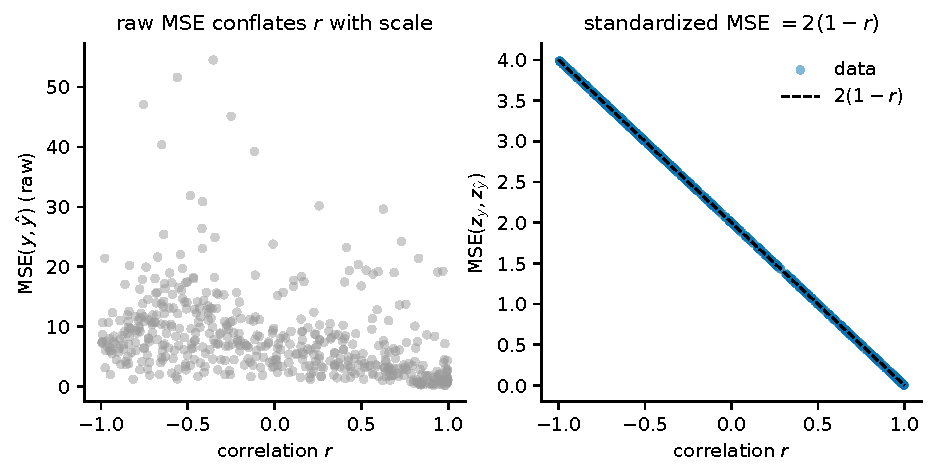
\includegraphics[width=\linewidth]{figures/fig1_geometry.pdf}}{}
\caption{Geometry of the standardized-MSE / Pearson identity (Proposition~\ref{prop:1}).}
\label{fig:geometry}
\end{figure}

\subsection{Affine calibration restores scale without changing rank}\label{sec:prop2}
Correlation is invariant to strictly increasing affine transformations of $\hat
y$: a model trained on $\mathcal{L}_{\mathrm{P}}$ controls the \emph{shape} of the
prediction but not its scale or offset. This is corrected exactly and cheaply.
\begin{proposition}\label{prop:2}
Let $p\in\mathbb{R}^n$ be raw predictions and $r=r(y,p)$. The affine map
$\tilde y = a\,p+b$ minimizing $\tfrac1n\sum_i (a p_i + b - y_i)^2$ has
\[
a^\star = \frac{\mathrm{cov}(y,p)}{\mathrm{var}(p)},\qquad
b^\star = \bar y - a^\star\,\bar p,\qquad
\mathrm{MSE}_{\min} = \sigma_y^2\,(1-r^2).
\]
If $a^\star>0$, the map is strictly increasing and hence preserves $r$, the
Spearman correlation, and every top-$k$/ranking quantity, while setting the
calibration slope to $1$ and intercept to $0$.
\end{proposition}
\begin{proof}
Ordinary least squares for a single predictor gives $a^\star,b^\star$ as stated;
the minimized residual variance of simple linear regression is
$\sigma_y^2(1-r^2)$. A strictly increasing transform preserves the order of $p$
and leaves correlation-type and rank-based statistics unchanged.
\end{proof}
We fit $(a^\star,b^\star)$ on held-out validation predictions (never on the test
set) and apply them to the test predictions. Isotonic regression provides a
monotone non-linear alternative when the raw-vs-true relationship is monotone but
curved. A positive affine map preserves $r$; a negative affine slope changes its
sign, and nonlinear isotonic calibration can change its magnitude. Calibration
can nonetheless improve RMSE, bias and slope (Figure~\ref{fig:simulation};
Section~\ref{sec:res-calibration}).

\begin{figure}[tbp]\centering
\IfFileExists{figures/fig2_simulation.pdf}{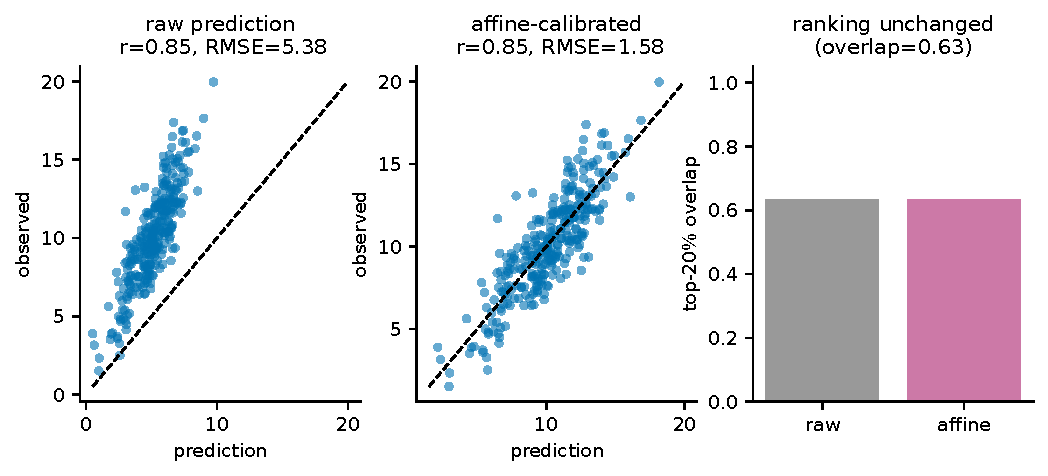
\includegraphics[width=\linewidth]{figures/fig2_simulation.pdf}}{}
\caption{Controlled simulation of Proposition~\ref{prop:2}: a well-correlated but
mis-scaled prediction (left) is corrected by affine calibration (middle) ---
RMSE falls while Pearson $r$ is unchanged --- and the top-$20\%$ selection
overlap is identical before and after (right).}
\label{fig:simulation}
\end{figure}

\subsection{Mini-batch versus global Pearson}\label{sec:prop3}
\begin{proposition}\label{prop:3}
For a partition of the data into batches $B_1,\dots,B_K$, the batch-averaged loss
$\tfrac1K\sum_k \bigl(1-r_{B_k}\bigr)$ is not equal to $1-r_{\mathrm{global}}$ in
general, because $r$ is a non-linear (ratio-of-moments) functional of the data.
Because the functional is nonlinear, neither equality nor a monotonic relation
between batch size and discrepancy is guaranteed without further assumptions.
\end{proposition}
A full-batch evaluation of $\mathcal{L}_{\mathrm{P}}$ optimizes the global
objective exactly; a large batch is an approximation, and smaller batches
optimize a noisier surrogate. A supporting experiment quantifies the practical
effect over the tested range.

\subsection{Multi-trait and group-aware variants}\label{sec:groupaware}
The loss extends naturally to $T$ traits, $\mathcal{L}=\tfrac1T\sum_{t=1}^T
(1-r_t)$ (or a weighted sum $\sum_t w_t(1-r_t)$), and to a group-aware objective
$\mathcal{L}=\tfrac1G\sum_{g=1}^G (1-r_g)$ where $g$ indexes environments, years,
families or sites --- aligning training with the within-environment correlation
that multi-environment breeding programs actually care about. As in
Proposition~\ref{prop:3}, neither variant equals the pooled global correlation.

\section{Materials and Methods}\label{sec:methods}

\paragraph{Datasets.} We use three public sources, for a total of \NUM{101}
trait--dataset combinations across \NUM{12} panels/sources spanning 10 species. (i) \emph{EasyGeSe}
\citep{quesada2025easygese}: a benchmark of ten species (barley, common bean,
lentil, maize, eastern oyster, pig, loblolly pine, rice, soybean and wheat)
providing genotypes, phenotypes and \emph{fixed} cross-validation partitions; the
maize set is the global genotype-by-environment competition panel
\citep{washburn2025maize}. (ii) The CIMMYT \emph{wheat} panel
\citep{crossa2010}: 599 lines, 1{,}279 DArT markers and grain yield in four
environments, analyzed as four outcomes. (iii) \emph{SoyNAM}
\citep{xavier2016soynam}: $\sim$5{,}500 recombinant inbred lines in 40 biparental
families, analyzed for four agronomic traits. Genotypes are coded as allele
dosages; preprocessing (unsupervised, no phenotype) applies a minor-allele
frequency filter ($\geq 0.01$), mean imputation, and a top-variance cap at
20{,}000 markers for the seven panels whose marker count exceeded 20{,}000
(barley, lentil, maize, oyster, pig, rice and soybean).
Table~\ref{tab:datasets} and Figure~\ref{fig:datasets} summarize the data.

\begin{table}[t]\centering
\caption{The 101 trait--dataset combinations across 12 panels/sources (10 species;
10 panels from EasyGeSe, plus CIMMYT wheat and SoyNAM). $n$ is the number of genotypes, $p$ the markers used
(after MAF filtering and the 20{,}000-marker variance cap), and GBLUP $r$ the mean
within-dataset predictive ability of GBLUP (a difficulty index).}\label{tab:datasets}
\begin{tabular}{lrrrrl}
\toprule
Species & $n$ & $p$ & traits & GBLUP $r$ & source\\
\midrule
rice & 352 & 20{,}000 & 36 & 0.46 & EasyGeSe \\
pine & 925 & 4{,}421 & 17 & 0.82 & EasyGeSe \\
wheatG & 371 & 12{,}546 & 16 & 0.59 & EasyGeSe \\
maize & 4421 & 20{,}000 & 6 & 0.83 & EasyGeSe \\
bean & 444 & 16{,}707 & 5 & 0.57 & EasyGeSe \\
lentil & 324 & 20{,}000 & 5 & 0.79 & EasyGeSe \\
soybeanNAM & 5487 & 4{,}401 & 4 & 0.71 & SoyNAM \\
wheat & 599 & 1{,}279 & 4 & 0.46 & BGLR/CIMMYT \\
barley & 1438 & 20{,}000 & 2 & 0.58 & EasyGeSe \\
oyster & 372 & 20{,}000 & 2 & 0.38 & EasyGeSe \\
pig & 1709 & 20{,}000 & 2 & 0.31 & EasyGeSe \\
soybean & 346 & 20{,}000 & 2 & 0.40 & EasyGeSe \\
\bottomrule
\end{tabular}

\vspace{2pt}
{\footnotesize\raggedright The count of 12 panels/sources (spanning 10 species)
treats related germplasm
sharing a common crop as distinct panels: wheatG (EasyGeSe) and wheat (CIMMYT) are
separate sources, as are soybean (EasyGeSe) and soybeanNAM (SoyNAM)
panels of the same species drawn from different sources.\par}
\end{table}

\begin{figure}[tbp]\centering
\IfFileExists{figures/fig3_datasets.pdf}{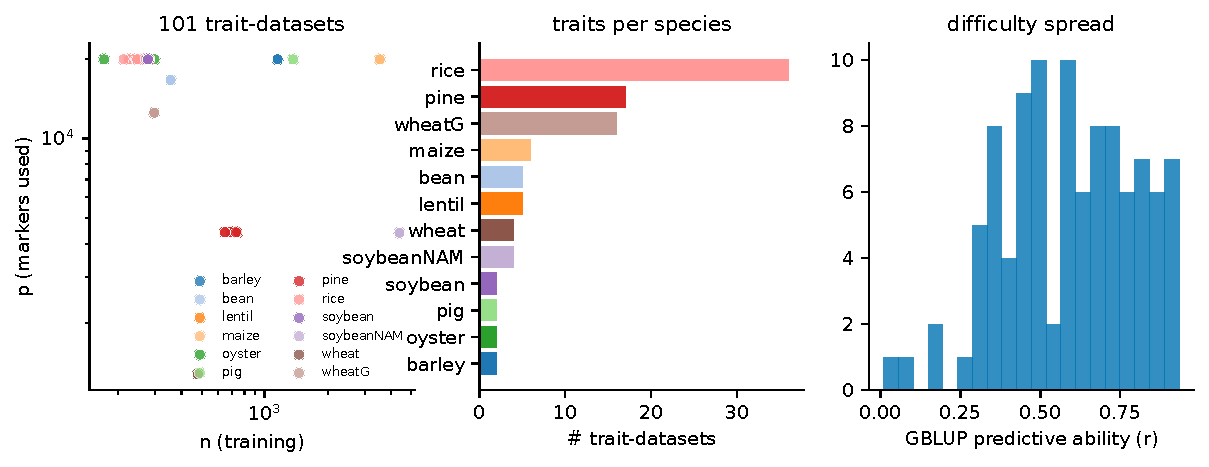
\includegraphics[width=\linewidth]{figures/fig3_datasets.pdf}}{}
\caption{Dataset map: size, dimensionality and predictability across species.}
\label{fig:datasets}
\end{figure}

\paragraph{Models.} The parametric baseline is GBLUP with REML-estimated variance
components, implemented in the spectral basis of the linear genomic kernel
$K=XX^\top/p$ and validated against the \texttt{rrBLUP} package
\citep{endelman2011} to floating-point precision (cross-implementation
correlation $1.0000$). We also include ridge regression as a linear baseline. The neural predictors
are a multilayer perceptron (MLP), a one-dimensional convolutional network over
ordered markers (1D-CNN), a light Transformer over marker patches, and four
protocol-matched, literature-inspired adaptations: DeepGS
\citep{ma2018deepgs}, DNNGP \citep{wang2023dnngp}, PNNGS \citep{pnngs2024}, and
SoyDNGP \citep{gao2023soydngp}. These are not exact reproductions: they retain
published motifs while using common dosage inputs, preprocessing, training and
evaluation. For the primary ablation, one configuration is selected per dataset
registry key and architecture under MSE and frozen across losses. EasyGeSe and
CIMMYT use one representative trait per panel and transfer it to the other
traits; the four SoyNAM phenotypes are separate registry keys and are tuned on
their own phenotype. The contrast changes only the loss conditional on the
configuration, but selection under MSE may favor MSE.

\paragraph{Loss functions.} We compare MSE; the standardized-MSE Pearson loss
$1-r$ (Proposition~\ref{prop:1}); a hybrid $\,(1-r)+\lambda\,\mathrm{MSE}\,$ with
$\lambda=0.1$; and a concordance-correlation loss $1-\rho_c$ \citep{lin1989},
which penalizes correlation, scale and offset jointly. The negative-Pearson and
explicit standardized-MSE forms are included in the numerical checks.

\paragraph{Calibration.} For every model and loss we report predictions under
three post-hoc maps: raw (identity), affine (Proposition~\ref{prop:2}) and
isotonic. Calibrators are fit on validation predictions only.

\paragraph{Cross-validation.} We use the fixed EasyGeSe partitions (5 folds
$\times$ 2 repeats $=$ 10 folds per trait) and repeated $K$-fold for wheat and
SoyNAM. Within each training fold an inner 80/20 split provides early-stopping and
calibration data; markers are standardized with training statistics only;
targets are standardized with training statistics for the neural networks and
predictions are returned in the original units. Neural networks early-stop on the
validation value of the loss being trained. The test fold is never used for
fitting, early stopping or calibration. Primary hyper-parameters, however, were
selected before outer CV on the full tuning phenotype described above, so
absolute performance is not a nested estimate. In a separate CIMMYT sensitivity,
MSE and Pearson each received the same eight-candidate bank inside five outer
folds using only environment-1 outer-training observations; configurations were
evaluated in four environments with three initialization seeds.

\paragraph{Evaluation metrics.} Predictive: Pearson $r$, Spearman $\rho$, RMSE,
MAE, $R^2$, mean bias, and the calibration slope and intercept (ideal $1$ and
$0$). Upper-tail ranking, at intensities $k\in\{5,10,15,20\}\%$: top-$k$ overlap,
precision@$k$, recall@$k$, NDCG@$k$ \citep{jarvelin2002ndcg}, selection
differential, mean phenotype of the selected, and relative efficiency (achieved
upper-tail differential divided by the oracle differential). Larger phenotypes
are always the target; these metrics are not interpreted as breeding gain when
lower or intermediate values are desirable.

\paragraph{Statistical analysis.} For each task, architecture and loss we first
average the ten fold values and form
$\Delta m=m_{\mathrm{loss}}-m_{\mathrm{MSE}}$. The pooled contrast averages the
seven architectures within task. The primary estimand gives equal weight to each
of 12 panels; a trait-weighted estimand is a sensitivity check. Confidence
intervals resample panels as clusters (20,000 replicates), and an exact two-sided
sign-flip test reverses all task contrasts within a panel together.
Leave-one-panel-out ranges assess influence. A corroborative mixed model of the
paired deltas contains loss, architecture, their interaction, panel as a blocking
factor and a random task intercept; a likelihood-ratio test compares models with
and without the interaction. Raw Pearson is the prespecified primary endpoint,
raw NDCG@$10$ is secondary, and RMSE is normalized by the test-fold phenotype
standard deviation after validation-fitted affine calibration. The nested-HPO
experiment covers MLP, CNN and Transformer only and is analyzed separately and descriptively because its environments,
folds and seeds are repeated measures from one wheat panel.

\paragraph{Implementation.} The framework is released as the Python package
\texttt{ccgp}, built on PyTorch \citep{paszke2019pytorch}, scikit-learn
\citep{pedregosa2011sklearn} and NumPy
\citep{harris2020numpy}, with the neural networks trained using the Adam optimizer
\citep{kingma2015adam}, deterministic split definitions and recorded tuned
configurations. The main campaign used one initialization per fold; only the
nested wheat sensitivity used three seeds. Analysis scripts validate the
90,900-row campaign and 1,080-row nested result files before producing tables
and machine-readable figure source data.

\section{Results}\label{sec:results}

\subsection{Numerical validation}\label{sec:res-numerical}
Across 80 simulated cases, the implemented Pearson loss, $1-r$, and one half of
the standardized MSE agreed to a maximum absolute difference of
$5.0\times10^{-8}$ (mean $7.4\times10^{-9}$). The affine residual identity in
Proposition~\ref{prop:2} agreed to $1.2\times10^{-15}$ over 200 cases. Both the
Pearson and concordance losses passed automatic gradient checks, and $-r$ and
$1-r$ had identical gradients. These checks establish numerical equivalence,
not empirical superiority.

\subsection{Headline result: correlation, calibration and selection separate}\label{sec:res-loss}

\ifdefined\GTHREE\else
\begin{figure}[tbp]\centering
\IfFileExists{figures/fig4_loss_comparison.pdf}{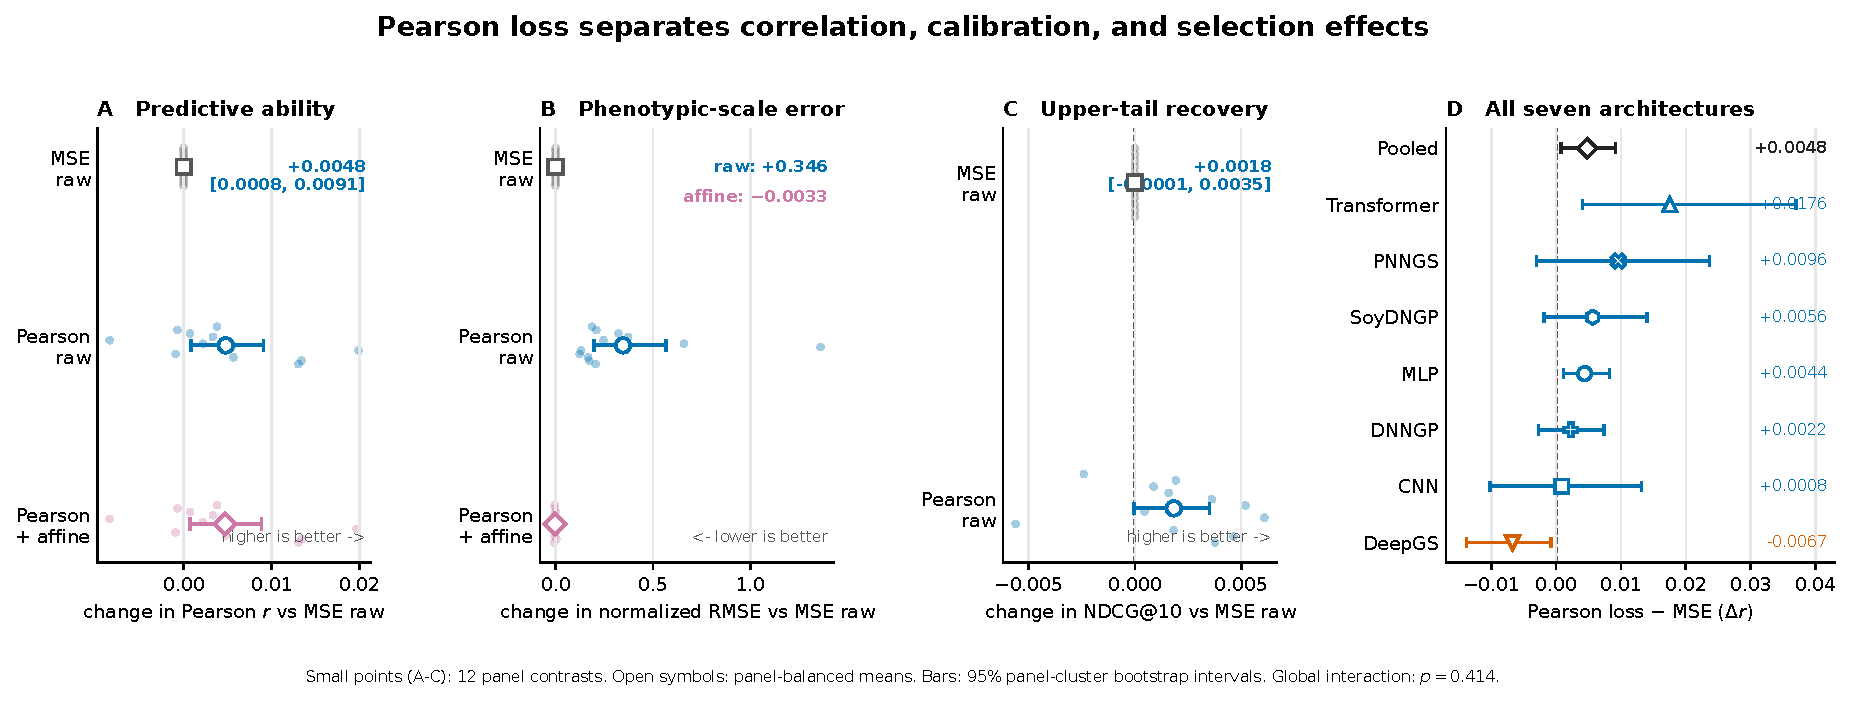
\includegraphics[width=\linewidth]{figures/fig4_loss_comparison.pdf}}{}
\caption{The paper's central comparison. Panels A--B compare the scale-aware
raw MSE baseline, the correlation-targeted but unscaled raw Pearson output, and
the validation-fitted affine Pearson output; Panel C compares raw MSE and raw
Pearson predictions for upper-tail recovery. Small points are contrasts for
each of 12 panels, open symbols are panel-balanced means, and bars are 95\%
panel-cluster bootstrap intervals. Raw Pearson predictions gain $0.0048$ in $r$
but lose $0.346$ in normalized RMSE; affine calibration retains a $0.0047$
correlation gain and changes normalized RMSE by $-0.0033$. The raw NDCG@$10$
change is only $+0.0018$. Panel D reports the Pearson-minus-MSE correlation
contrast, interval and exact point estimate for
the pooled result and every neural architecture in the main benchmark. Folds
were averaged within 101 tasks and architectures within task before panels were
weighted equally.}
\label{fig:loss}
\end{figure}
\fi

Figure~\ref{fig:loss} summarizes the practical sequence. Relative to the
MSE-trained raw baseline, Pearson-trained raw predictions gained $0.0048$ in
correlation but increased normalized RMSE by $0.346$ (95\% panel-cluster
bootstrap interval $[0.1965,0.5675]$), because correlation training does not
identify scale or offset. Validation-fitted affine calibration retained nearly
all of the correlation gain ($+0.0047$) and brought normalized RMSE back to the
MSE baseline ($-0.0033$, $[-0.0062,0.0000]$). Thus the headline is not that
Pearson replaces MSE on every criterion: it slightly improves the target
correlation, a separate calibration step is needed for phenotypic-scale
predictions, and the decision-level effect must be checked directly.

The final grid contained 90,900 rows: seven neural architectures, four losses,
101 tasks, ten test folds and three calibration maps, plus GBLUP and ridge
baselines. All architectures covered the same 101 tasks. After folds were
averaged, the panel-balanced Pearson-minus-MSE contrast for raw test correlation
was $\Delta r=+0.0048$ (95\% panel-cluster bootstrap interval
$[0.0008,0.0091]$). Seventy-eight of 101 task-level pooled
contrasts were positive. An exact test that flipped the signs of all tasks
within each panel gave $p=0.052$, appropriately reflecting that only 12 panels,
not 707 independent experiments, were observed. Weighting every trait equally
instead produced $+0.0101$ ($[0.0028,0.0158]$), showing that the estimate is
sensitive to the many traits contributed by rice, pine and wheatG.

The hybrid and CCC losses gave panel-balanced $\Delta r$ values of $+0.0055$
($[0.0010,0.0100]$) and $+0.0078$ ($[0.0022,0.0139]$), respectively. Figure~\ref{fig:loss}D
reports all seven architecture-specific Pearson contrasts and intervals. The
Transformer has the largest positive estimate ($+0.0176$), while DeepGS is a
negative counterexample ($-0.0067$); PNNGS and SoyDNGP are positive but
uncertain, MLP shows a smaller positive estimate, and DNNGP and CNN lie near
zero. The apparent spread is descriptive: the global loss-by-architecture test
is inconclusive ($\chi^2_{12}=12.40$, $p=0.414$). The four named networks are
literature-inspired adaptations, not exact reproductions of the published systems.

\subsection{Ranking and scale}\label{sec:res-selection}
Pearson training changed panel-balanced raw NDCG@$10$ by only $+0.0018$
($[-0.0001,0.0035]$) and upper-tail overlap by $+0.0033$
($[-0.0010,0.0069]$). CCC gave the largest, still small, NDCG contrast
($+0.0034$, $[0.0015,0.0056]$). These quantities recover the highest observed
phenotypes; because trait desirability was not harmonized, they must not be read
as realized breeding gain for traits where lower values are preferred. Ridge
and GBLUP retained the best mean ranks for both Pearson and NDCG@$10$. The weak
ranking response is therefore an empirical result in its own right: a measurable
gain in global predictive ability did not substantially change which candidates
would be recovered by the upper-tail rule used here.

Affine-calibrated NRMSE, defined as RMSE divided by the test-fold phenotype
standard deviation, was essentially unchanged by Pearson training
($-0.0011$, $[-0.0036,0.0015]$) or the hybrid loss ($-0.0018$,
$[-0.0041,0.0006]$). CCC produced $-0.0028$ ($[-0.0054,-0.0003]$), a very small
normalized-error reduction. Absolute RMSE values were not pooled across traits
because their measurement units differ.

\subsection{Calibration}\label{sec:res-calibration}

\ifdefined\GTHREE\else
\begin{figure}[tbp]\centering
\IfFileExists{figures/fig5_calibration.pdf}{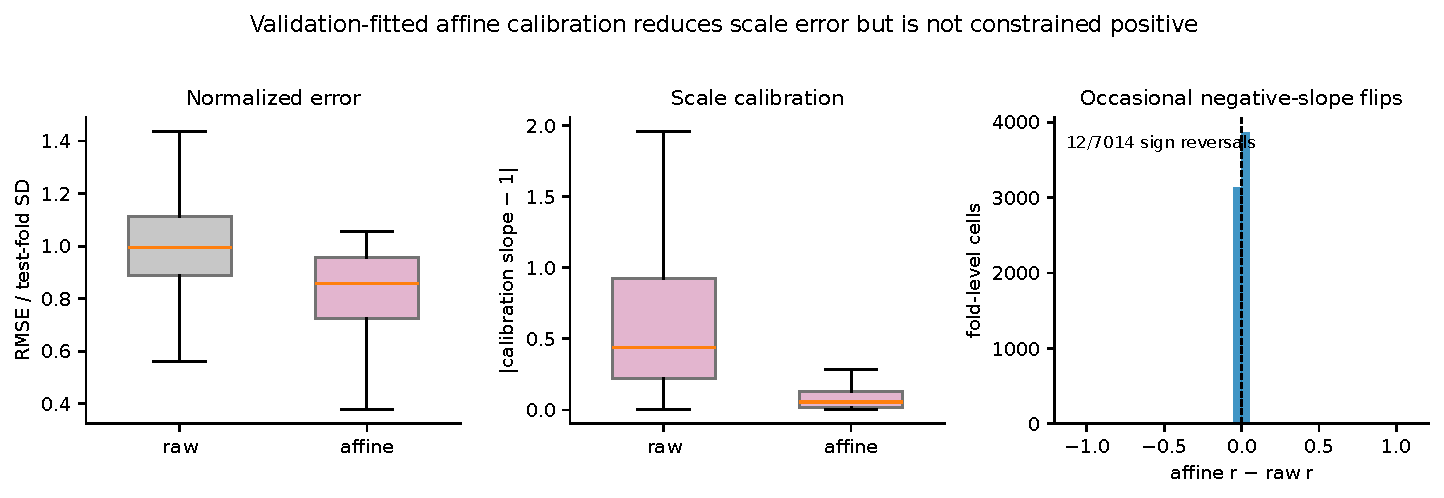
\includegraphics[width=\linewidth]{figures/fig5_calibration.pdf}}{}
\caption{Validation-fitted affine calibration for Pearson-trained networks.
Boxplots summarize 707 task--architecture means (outliers omitted visually);
the histogram uses 7,014 fold-level cells with finite raw and affine
correlations. Calibration reduced normalized error and slope deviation, but 12
folds (0.17\%) had a validation-fitted negative slope that reversed the sign of
test-set correlation.}
\label{fig:calibration}
\end{figure}
\fi

Across Pearson-trained networks, mean RMSE fell from 10.54 to 7.99 after affine
calibration and the median calibration slope moved from 0.918 to 0.957. These
raw-unit averages are descriptive only. A positive affine map preserves ranks,
but the implementation used the unconstrained least-squares slope estimated on
validation data. Among 7,014 comparable fold cells, 12 (0.17\%) therefore
reversed the sign of test correlation. Loss comparisons for correlation and upper-tail recovery use raw predictions.
Figure~\ref{fig:loss} additionally audits raw versus affine correlation to check
that calibration retains the gain. Scale outcomes use affine predictions.

\subsection{Loss-specific HPO and seed sensitivity}\label{sec:res-nested}

\ifdefined\GTHREE\else
\begin{figure}[tbp]\centering
\IfFileExists{figures/fig6_meta.pdf}{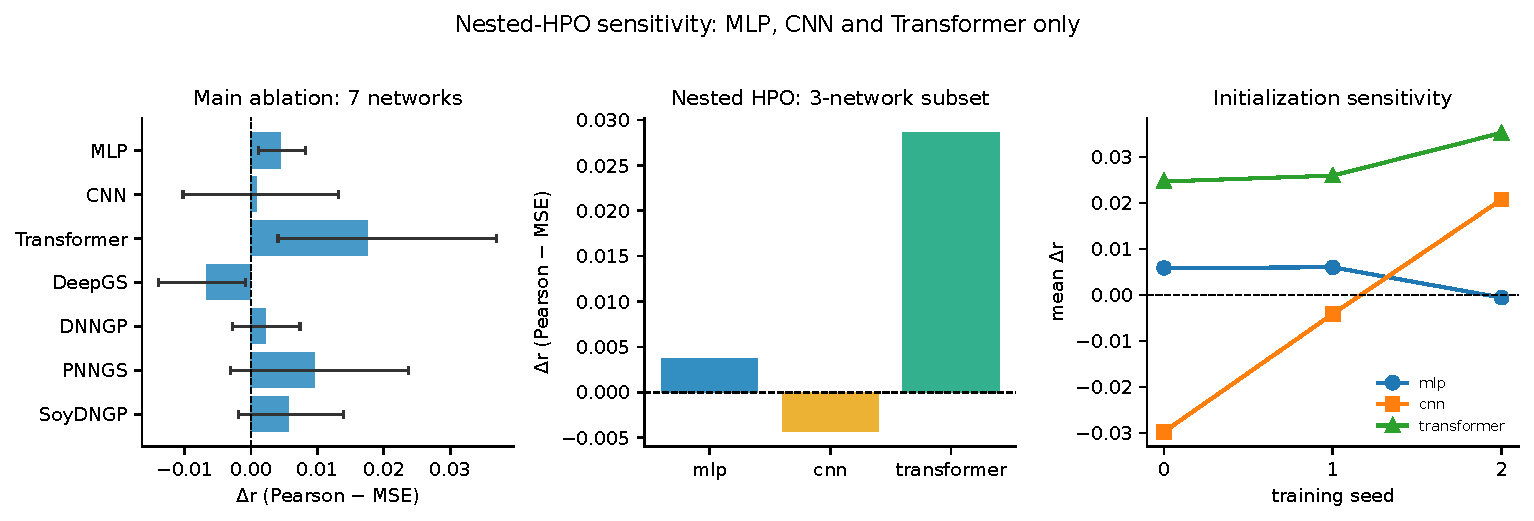
\includegraphics[width=\linewidth]{figures/fig6_meta.pdf}}{}
\caption{Sensitivity to tuning and initialization. The shared-HPO panel shows
panel-balanced effects for all seven networks in the 101-task benchmark. The
nested-HPO and seed panels contain only MLP, CNN and Transformer because
loss-specific nested tuning was run only for these three generic architectures;
the four literature-inspired networks were not evaluated in this sensitivity.
Nested means cover four CIMMYT wheat environments, five outer folds and three
seeds; configurations were selected separately for MSE and Pearson using only
environment-1 observations in each outer-training set. The repeated wheat
outcomes are not independent replications and no confirmatory $p$-value is assigned.}
\label{fig:meta}
\end{figure}
\fi

The nested sensitivity contained 1,080 prediction rows. It was run only for
MLP, CNN and Transformer; DeepGS, DNNGP, PNNGS and SoyDNGP therefore have no
loss-specific nested-HPO result, rather than an omitted result (Figure~\ref{fig:meta}).
Across the three tested architectures, loss-specific Pearson tuning changed raw $r$ by $+0.0093$ on
average. Estimates were $+0.0286$ for the Transformer, $+0.0038$ for the MLP,
and $-0.0044$ for the CNN. Corresponding NDCG@$10$ contrasts were $+0.0069$,
$+0.0071$, and $-0.0060$. CNN's mean $\Delta r$ moved from $-0.0297$ to
$-0.0041$ to $+0.0207$ across seeds 0--2; Transformer remained positive
($+0.0246$, $+0.0259$, $+0.0352$). Thus objective-specific tuning supports the
Transformer signal but also demonstrates initialization uncertainty that the
single-seed main campaign cannot quantify.


\section{Discussion}\label{sec:discussion}

\subsection{A valid objective with a modest empirical effect}
The algebraic result is exact: minimizing standardized MSE maximizes Pearson
correlation. The empirical result is more restrained. Once all seven networks
are evaluated on the same 101 tasks and panels are equally weighted, Pearson
training improves $r$ by about five thousandths. The cluster-bootstrap interval
is positive, but an exact 12-panel sign-flip test lies at the conventional
threshold. The raw Pearson outputs pay a large scale penalty; validation-fitted
affine calibration removes it while leaving the correlation gain essentially
intact. NDCG changes are smaller still. This sequence---align the objective,
then restore scale---and the distinction between mathematical alignment and
modest practical gain are the paper's main findings.

Trait weighting matters. A trait-weighted analysis gives twice the
panel-balanced effect because rice, pine and wheatG contribute many phenotypes.
Neither estimand is intrinsically wrong: the first describes an average listed
trait and the second an average panel. We use panel balance for the headline to
avoid allowing heavily phenotyped resources to determine a cross-panel claim,
and report both for transparency.

\subsection{Architecture heterogeneity is suggestive, not universal}
The Transformer repeatedly shows the largest positive estimate, including after
loss-specific nested tuning. MLP gains are small, CNN is near zero after panel
balance, and the DeepGS-inspired network becomes worse under Pearson training.
This counterexample rules out a universal optimization advantage. At the same
time, the omnibus loss-by-architecture interaction is not significant, so the
apparent ordering should be treated as hypothesis-generating rather than as a
formal taxonomy of networks. Possible mechanisms include different curvature,
normalization and early-stopping behavior, but the present benchmark does not
identify them.

The four named systems are protocol-matched, literature-inspired adaptations.
DeepGS retains a marker convolution/dense motif but adds batch normalization;
DNNGP is genotype-only and uses PCA rather than reproducing its complete
multi-omic setting; PNNGS retains parallel residual kernels but changes the
stem, pooling and validation protocol; and SoyDNGP converts dosage vectors to a
96$\times$96 one-channel representation rather than the published
206$\times$206$\times$3 encoding. Their results evaluate whether these motifs
respond to the loss under one common protocol, not whether the original papers
would reproduce identically.

\subsection{Correlation, calibration and upper-tail recovery}
Correlation is invariant to positive affine transformations, making scale
calibration a separate problem. Validation-fitted affine calibration reduced
normalized error in aggregate, but unconstrained least squares occasionally
estimated a negative slope and reversed rankings. A production implementation
should constrain the slope to be positive or fall back to an intercept-only
map. We avoided this ambiguity by using raw outputs for correlation and ranking
and affine outputs only for scale outcomes.

The upper-tail metrics answer a narrower question than biological selection.
They quantify recovery of the largest observed phenotypes. Some disease,
maturity and moisture traits favor lower or intermediate values, and the public
metadata did not provide a uniform desirability direction. Consequently these
metrics cannot establish breeding utility without trait-specific economic
weights and target directions. Their weak improvement nevertheless shows that a
small gain in global correlation need not translate into a substantial change
in the selected set, consistent with earlier ranking-based critiques
\citep{ornella2014,blondel2015}.

\subsection{What the HPO comparison does and does not show}
The main experiment is a controlled shared-configuration ablation. For each
panel and architecture, a configuration selected under MSE on one representative
trait was transferred to all traits and frozen across losses. This isolates the
training objective conditional on that configuration, but it can favor MSE and
uses the tuning phenotype before outer evaluation; it is not nested
performance estimation. The separate CIMMYT experiment selects MSE and Pearson
configurations inside each outer-training set from identical candidate banks.
Its Transformer result is directionally consistent with the main analysis, but
the experiment tunes on environment 1, transfers to four correlated wheat
environments, and covers only three architectures. It is a sensitivity analysis,
not a second general benchmark.

\subsection{Limitations and future work}
The main campaign uses one neural initialization per fold. The three-seed wheat
analysis shows that this is a material limitation, especially for CNN. Future
work should repeat all task--architecture cells over seeds, nest tuning within
every outer fold and phenotype, and record the full HPO trial ledger rather than
only selected configurations. With only 12 panels, resampling uncertainty also
remains coarse even though folds and architectures are not treated as independent
replicates.

The marker filter, imputation and variance cap were fitted transductively on the
full genotype matrix but without phenotypes; fold-specific standardization was
then fitted on training individuals. Binary, ordinal and continuous phenotypes
were analyzed together for breadth, although Gaussian calibration and RMSE have
different meanings across these scales. Constant or nearly constant test folds
also generated missing correlations, concentrated in rice seed color. These
limitations motivate stratified future benchmarks.

Finally, the benchmark compares objective functions, not every possible neural
architecture, and linear baselines remain strongest by mean rank. The practical
recommendation is therefore conservative: try Pearson or CCC as a paired
objective ablation when correlation is the operational endpoint; retain MSE and
linear baselines; calibrate separately when phenotypic scale matters; and verify
the actual trait-specific selection decision rather than inferring it from $r$.


\section{Conclusion}
A standardized-MSE Pearson loss aligns neural-network training with the
predictive-ability metric used throughout genomic prediction; because correlation
is scale-free, a separate calibration step or a scale-aware objective is needed
when calibrated phenotypic values matter; and global correlation should be
complemented by decision-specific metrics. Empirically, across 101 trait--datasets the average
benefit is small, sensitive to panel weighting, and not uniform across
architectures. The clearest descriptive signal occurs for the Transformer,
while DeepGS provides a negative counterexample, and no neural loss unseated
GBLUP or ridge on mean rank. Together, these results provide a practical
framework for separating objective alignment, phenotypic calibration and
decision-level evaluation in neural genomic prediction; Pearson or CCC should be
viewed as objective-specific alternatives to test alongside MSE rather than as
universal replacements.

\section*{Data availability}
All datasets are public: EasyGeSe (Zenodo, DOI \texttt{10.5281/zenodo.15348871}), the CIMMYT wheat panel
(\texttt{BGLR} R package \citep{perez2014bglr}) and SoyNAM (\texttt{SoyNAM} R package). Code, fixed
cross-validation partitions, tuned configurations and a recorded runtime manifest are
released as the \texttt{ccgp} package, with source at
\url{https://github.com/GBeurier/gs-loss} (a versioned archive will be
deposited at Zenodo, DOI to be assigned). All datasets used in the reported
benchmark are public and download automatically. Supporting Information (File~S1,
\texttt{supplement.pdf}) documents the architecture adaptations, complete paired
contrasts, missingness, HPO provenance, calibration, mean ranks and nested wheat
sensitivity. Machine-readable source tables accompany every data-driven figure.

\bibliographystyle{apalike}
\bibliography{refs}



\end{document}
